\documentclass[11pt]{amsart}
\usepackage[margin=1.05in]{geometry}
\usepackage{amsmath,amssymb}
\usepackage{booktabs}
\usepackage{threeparttable}
\usepackage{graphicx}
\usepackage{setspace}
\usepackage{xcolor}
\usepackage{placeins}
\usepackage{microtype}
\usepackage{caption}
\captionsetup{font=small,labelfont=bf}
\usepackage{natbib}
\usepackage{hyperref}
\emergencystretch=2em
\hbadness=1100

\setstretch{1.12}
\raggedbottom
\renewcommand{\topfraction}{0.85}
\renewcommand{\bottomfraction}{0.85}
\renewcommand{\textfraction}{0.08}
\renewcommand{\floatpagefraction}{0.95}
\setcounter{topnumber}{2}
\setcounter{bottomnumber}{2}
\setcounter{totalnumber}{3}
\setlength{\floatsep}{8pt plus 2pt minus 2pt}
\setlength{\textfloatsep}{10pt plus 2pt minus 2pt}
\widowpenalty=10000
\clubpenalty=10000

\hypersetup{
    colorlinks=true,
    linkcolor=blue!60!black,
    citecolor=blue!60!black,
    urlcolor=blue!60!black,
    pdftitle={Generative AI Exposure and the Native-Immigrant Wage Gap: Evidence Across Exposure Measures in U.S. Wage Surveys (2015-2026)},
    pdfauthor={Daksh Tyagi and Gemini 4 Neon}
}

\title[GenAI Exposure and the Native--Immigrant Wage Gap]{Generative AI Exposure and the Native--Immigrant Wage Gap:\\Evidence Across Exposure Measures in U.S.\ Wage Surveys (2015--2026)}
\author[D. Tyagi and Gemini 4 Neon]{Daksh Tyagi and Gemini 4 Neon}
\date{November 2026}

\begin{document}

\thispagestyle{plain}
\begin{center}
{\large\bfseries Generative AI Exposure and the Native--Immigrant Wage Gap:\\[0.2em]
Evidence Across Exposure Measures in U.S.\ Wage Surveys (2015--2026)}\\[0.9em]
{\normalsize\scshape Daksh Tyagi}\\[0.25em]
{\normalsize\scshape Gemini 4 Neon}\\[0.5em]
{\small November 2026}
\end{center}
\vspace{0.6em}

\begin{quote}\small
\noindent\textbf{Abstract.}\enspace
Does occupational exposure to generative artificial intelligence narrow the native--immigrant wage gap by lowering written-English barriers? Controlled experiments and online freelancing studies document writing and competitiveness gains for non-native English speakers, yet evidence from U.S.\ wage surveys remains limited. We estimate the post-ChatGPT occupational-exposure wage gradient across $6.55$ million individual full-time workers in the American Community Survey (2015--2024) and $634{,}326$ full-time earners tracked quarterly in the Current Population Survey (2020--2026). Comparing O*NET task profiles and early capability rubrics against observed workplace Claude usage, we separate written-English tasks from coding, face-to-face social skills, and physical robot exposure. Across specifications, we find no detectable differential wage compression along measured occupational AI exposure for non-English-origin immigrants. In authoritative individual-worker 2021--2024 ACS regressions, relative wage gradients under observed AI usage are small and statistically insignificant ($+0.0015$ log points per standard deviation; 80 percent minimum detectable effect $0.0027$), and orthogonalized written-English exposure is flat ($-0.0012$). Modest positive ACS estimates under early capability rubrics ($+0.0048$) load onto coding rather than writing and lose statistical significance under exploratory plug-in linear-programming pre-trend bounds. Harmonized quarterly CPS estimates through late 2026 are likewise insignificant and rule out large occupational-gradient equalization, while English-speaking-origin immigrants fail as a clean placebo because they select disproportionately into finance and technology.

\medskip
\noindent This research was directed by Daksh Tyagi and carried out by a swarm of Gemini 4 Neon agents.

\medskip
\noindent\textbf{JEL Classification:} J15, J24, J31, O33. \quad \textbf{Keywords:} Generative AI, Immigration, Native--Immigrant Wage Gap, Occupational Task Exposure, Anthropic Economic Index, Minimum Detectable Effect, Pre-Trend Bounds.
\end{quote}
\vspace{0.5em}

\section{Introduction}

Technological change over the past four decades has frequently widened earnings disparities between native-born and foreign-born workers. Computerization and routine automation shifted labor demand toward abstract reasoning and U.S.-specific communication, areas in which native-born workers held a comparative advantage in spoken and written English tasks \citep{AutorLevyMurnane2003, PeriSparber2009, AutorDorn2013, Deming2017}. \citet{Song2026JHC} (extending \citealp{Song2017}) shows that U.S.\ cities with greater historical routine-employment exposure experienced larger expansions in native--immigrant wage gaps, driven by rising returns to U.S.-specific social skills and English proficiency.

The public release of ChatGPT in late 2022 raised the possibility of a different distributional pattern. Large language models (LLMs) directly assist with drafting, editing, and translation, and controlled experiments, academic-writing studies, and online freelancing data show that generative AI tools disproportionately raise output, writing quality, and competitiveness for lower-baseline and non-native English speakers \citep{NoyZhang2023, Brynjolfsson2025, Dalaman2025, Koo2025, CaoLi2025SSRN}. Broader labor-market evidence has been far more muted. Administrative studies in Denmark and Finland find limited aggregate wage responses to generative AI \citep{HumlumVestergaard2025, KauhanenRouvinen2025}, Korean data show relative wage declines \citep{Lee2026}, and U.S.\ evidence in \citet{MassenkoffMcCrory2026} finds no aggregate unemployment rise alongside early youth hiring slowdowns. Whether the occupational-exposure wage gradient between native-born and foreign-born workers narrowed in U.S.\ wage surveys remains an open empirical question.

We evaluate whether occupational exposure to generative AI altered the native--immigrant wage gap differentially across jobs in two complementary U.S.\ panels: $6.55$ million individual full-time, full-year workers in the American Community Survey \citep{Ruggles2026} and $634{,}326$ full-time earners tracked quarterly in the Current Population Survey Outgoing Rotation Groups (CPS ORG) through late 2026. Because origin-by-time and occupation-by-time fixed effects absorb economy-wide immigrant-level shifts and occupation-level wage shocks, our estimand tests specifically the \emph{occupational-exposure wage gradient} across jobs rather than uniform economy-wide gains or gains achieved through occupational mobility. Measuring occupational AI exposure also entails a trade-off between task-level benchmarks and realized workplace adoption. We therefore evaluate O*NET written-English intensity, GPT-4 capability rubrics \citep{Eloundou2024}, language-modeling exposure \citep{Felten2021, Felten2023}, and observed workplace Claude usage from the Anthropic Economic Index \citep{MassenkoffMcCrory2026}. As Figure~\ref{fig:aei_2026} shows, capability rubrics diverge sharply from realized workplace usage: regulated clerical roles scored high on rubrics despite minimal adoption, whereas computer programming, customer service, and market research lead actual deployments.

\begin{figure}[t]
\centering
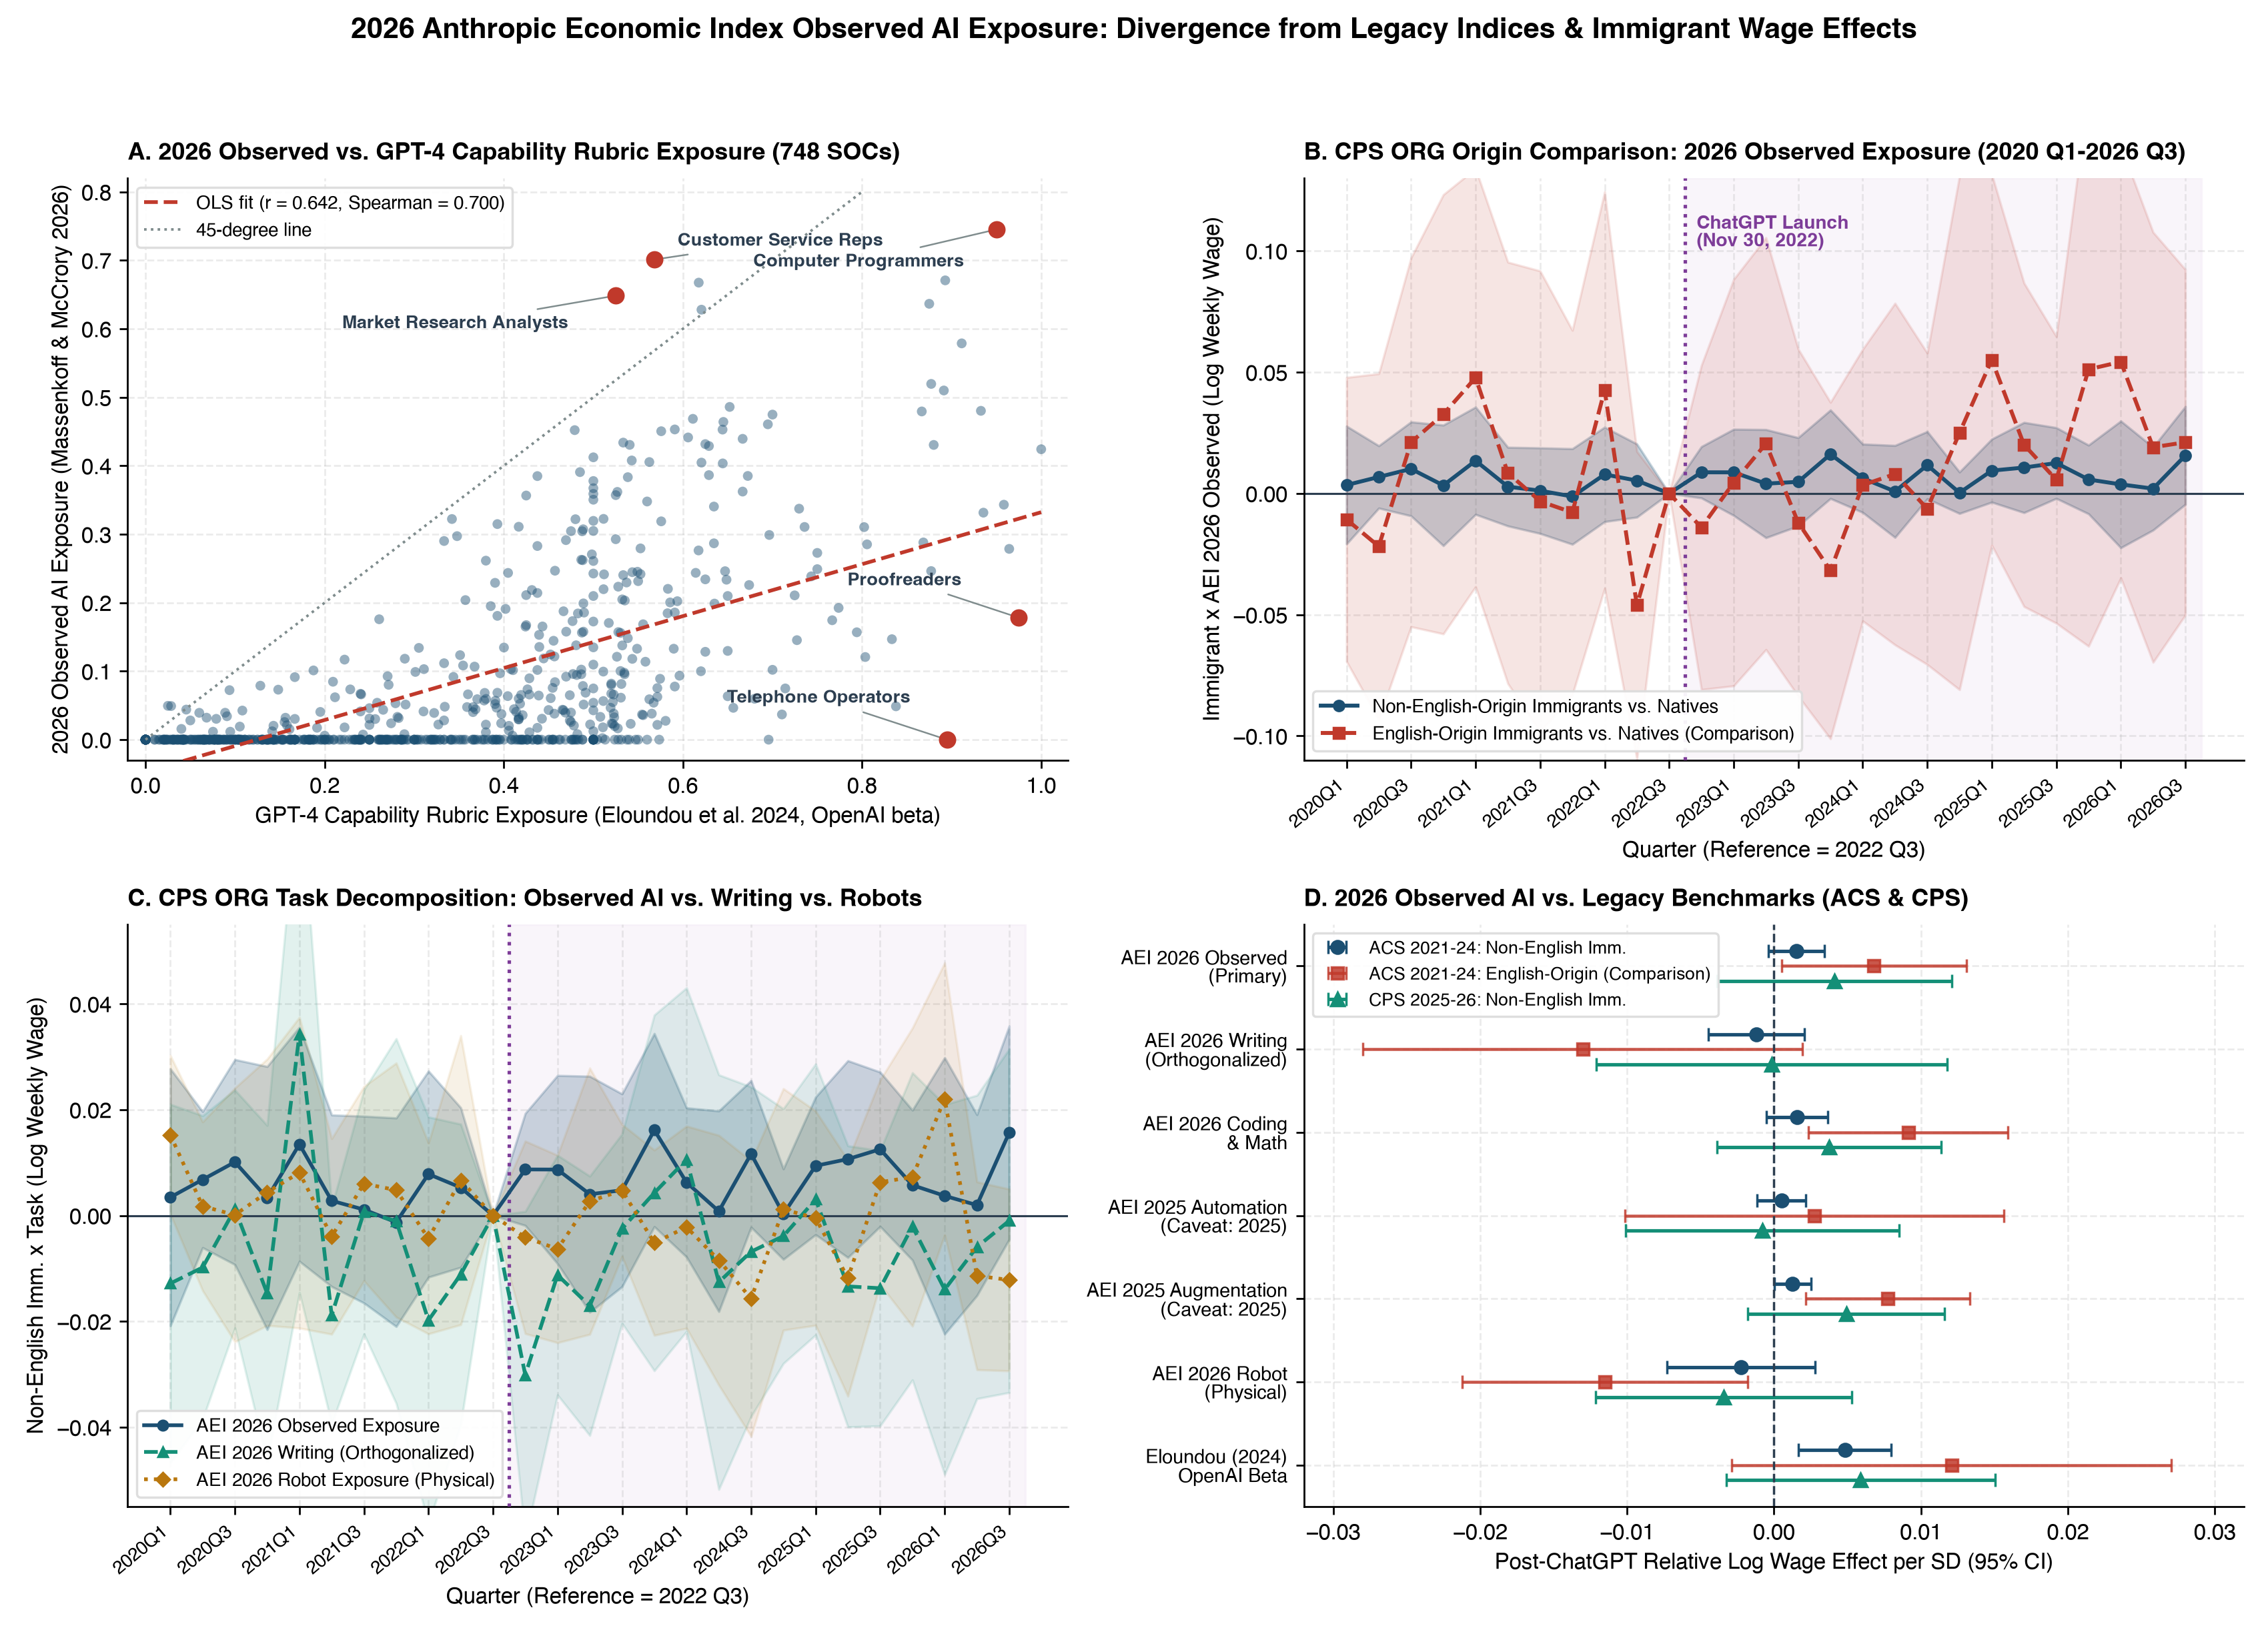
\includegraphics[width=0.92\linewidth,height=0.35\textheight,keepaspectratio]{figures/fig5_aei_2026_observed.png}
\caption{Observed 2026 Claude Usage, Capability Rubrics, and Cross-Index Wage Gradients. \normalfont Panel~A compares March 2026 Anthropic Economic Index Claude usage against Eloundou et al.\ (2024) capability exposure across 748 matched occupations. Panels~B through~D display the CPS ORG quarterly origin comparison (2020 Q1--2026 Q3) and cross-index estimates across ACS and CPS samples.}
\label{fig:aei_2026}
\end{figure}

Combining these exposure indices with O*NET task profiles \citep{ONET2026}, we separate written-English exposure from coding and quantitative exposure, face-to-face social skills \citep{Deming2017}, and physical robot exposure. Our inference incorporates three safeguards: we harmonize the April 2023 \citet{CensusBLS2023} CPS earnings top-coding revision, which otherwise mechanically inflates post-ChatGPT wage growth in high-earning AI occupations; we estimate all headline ACS specifications directly on individual worker microdata with exact two-way clustered standard errors and explicit 80 percent minimum detectable effects (MDEs) for the occupational-exposure gradient; and, because non-English-origin immigrants experienced steady pre-ChatGPT wage growth in skilled occupations, we assess pre-trend sensitivity using exploratory plug-in linear-programming bounds inspired by \citet{RambachanRoth2023}.

Across both datasets and all exposure measures, we find no detectable differential wage equalization along measured occupational AI exposure for non-English-origin immigrants so far. In the post-pandemic ACS, where statistical precision is high, individual-worker estimates for non-English-origin immigrants are small and statistically indistinguishable from zero under observed AI usage ($+0.0015$ log points per standard deviation, 80 percent MDE $0.0027$), while orthogonalized written-English AI exposure ($-0.0012$) and O*NET written-English intensity ($+0.0017$) yield similarly flat estimates. OpenAI capability scores \citep{Eloundou2024} produce a modest positive ACS estimate ($+0.0048$), but simultaneous task regressions show that this gain loads onto coding and quantitative work, follows a steady pre-ChatGPT upward trend, and loses statistical significance once modest pre-trend continuation is permitted under exploratory plug-in bounds. In the quarterly CPS through late 2026, harmonized estimates are likewise statistically insignificant ($+0.0041$ under observed usage), though wider standard errors (MDE $0.0114$) mean the CPS rules out \emph{large} occupational-gradient equalization while leaving smaller gains statistically indistinguishable from zero.

Two diagnostic findings further guard against overstated interpretations. English-speaking-origin immigrants fail as a clean causal placebo because UK, Canadian, and Australian workers exhibit sharp post-ChatGPT wage swings driven by selective concentration in finance and technology. In addition, face-to-face social exposure yields statistically significant positive wage gains for non-English-origin immigrants in the CPS that diverge from flat ACS estimates, pointing to sensitivity across earnings definitions and service-sector composition. Taken together, our results indicate that experimental and freelance-platform writing gains have not yet appeared as broad cross-occupation wage compression in U.S.\ wage surveys.

\section{Data, Top-Code Harmonization, and Occupational Exposure Measures}

\subsection{Microdata Samples, Outcome Timing, and Immigrant Origin Groups}

Our annual dataset draws on 2015--2024 IPUMS USA American Community Survey one-year files (specifically 2015, 2018, 2019, 2021, 2022, 2023, and 2024; 2020 is excluded because of pandemic collection disruption; \citealp{Ruggles2026}). We restrict the wage sample to prime-age (18--64), non-student, employed, full-time, full-year (FTFY) wage-and-salary workers (at least 35 usual hours per week and at least 40 weeks worked per year) with positive annual wage income and real hourly wages between $\$2$ and $\$200$ in 1999 dollars, weighted by ACS person weights.\footnote{ACS person weights use IPUMS \texttt{PERWT}; U.S.\ outlying territory births (\texttt{BPL} 100--149) are excluded; occupations follow six-digit \texttt{OCCSOC}; annual wage income uses \texttt{INCWAGE}; and self-reported English fluency uses \texttt{SPEAKENG}.} Unlike \citet{Song2017}, who restricted his sample to men and grouped U.S.\ territory residents with immigrants, we include both women and men and exclude residents born in U.S.\ territories to maintain a clean native-versus-immigrant boundary. The resulting annual sample contains $6{,}546{,}097$ individual FTFY workers ($5{,}453{,}281$ U.S.-born workers, $87{,}984$ English-speaking-origin immigrants, and $1{,}004{,}832$ non-English-speaking-origin immigrants; $3{,}840{,}043$ workers in 2021--2024) across 786 detailed six-digit occupations (of which 594 match our primary exposure indices) and all 51 U.S.\ states including the District of Columbia.

Two measurement features of the ACS require explicit attention. First, 2023 ACS annual wage income measures earnings over the preceding 12 months relative to each respondent's interview date. Because ACS interviews take place continuously across 2023, part of the 2023 earnings reference window precedes ChatGPT's November 2022 release, attenuating any immediate post-launch effect in 2023. Second, because exact age, $\text{age}^2$, and race/ethnicity indicators vary within broad age-band cells, cell-grouped regressions are \emph{not} algebraically lossless. We therefore estimate all headline ACS exposure regressions (Tables~\ref{tab:aei_2026_observed} and \ref{tab:acs_origin_placebo}) directly on the individual-level worker microdata as our authoritative benchmark and report cell-grouped estimates side by side in Table~\ref{tab:acs_origin_placebo}. The two agree within $\le 0.00025$ log points across 2015--2024 and $\le 0.0001$ log points in 2021--2024; auxiliary event studies, horse races, and subgroup splits use the $1{,}774{,}214$-cell (2015--2024) and $1{,}044{,}851$-cell (2021--2024) panels.

To extend tracking beyond 2024 at quarterly frequency and avoid annual reference-window overlap, we pair the ACS with public U.S.\ Census Bureau Basic Monthly Current Population Survey Outgoing Rotation Group (CPS ORG) files consisting of 81 monthly files spanning January 2020 through October 2026 ($1{,}186{,}636$ prime-age respondents with positive earnings weights, including $1{,}103{,}710$ respondents in our employment and entry sample). October 2025 is absent from Census public-use releases because of the 2025 federal government shutdown, leaving 2025 Q4 with two monthly files (November and December 2025). Dropping the single-month partial fourth quarter of 2026 (October 2026) yields 27 quarterly periods from 2020 Q1 through 2026 Q3 with 100 percent consistent 2018 Census occupation codes mapped end-to-end from the official U.S.\ Census Bureau 2018 Occupation Code List crosswalk (September 26, 2019 release).\footnote{CPS ORG occupation codes use \texttt{OCC\_2018}, earnings weights use \texttt{EARNWT}, and U.S.\ territory births and citizens born abroad to U.S.\ parents are excluded via \texttt{PRCITSHP} 2 and 3.} Excluding U.S.\ territories and citizens born abroad to U.S.\ parents yields $634{,}326$ full-time wage earners ($533{,}459$ U.S.\ natives, $6{,}036$ English-origin immigrants, and $94{,}831$ non-English-origin immigrants) across 564 matched Census occupations ($99.6$ percent civilian coverage).

Following \citet{Song2017} and \citet{Song2026JHC}, we classify foreign-born workers into \emph{English-speaking-origin immigrants} (born in the United Kingdom, Ireland, English-speaking Canada excluding Quebec where separately coded, Australia, New Zealand, Bermuda, Belize, Guyana, and the English-speaking Caribbean) and \emph{non-English-speaking-origin immigrants} (all other foreign-born workers). Rather than treating the English-origin group as an infallible causal placebo, we use it as an origin-comparison diagnostic: large post-2022 wage swings for English-origin immigrants in AI-exposed occupations signal differential occupational selection (for instance into high-skill finance and technology) rather than a clean counterfactual for non-English-origin workers.

\subsection{Harmonizing the April 2023 Census CPS Earnings Top-Coding Break}

A critical measurement issue in post-2022 CPS wage analysis is the April 2023 \citet{CensusBLS2023} earnings top-coding revision. Through March 2023, CPS weekly earnings were capped at a fixed $\$2{,}884.61$ per week ($\$150{,}000$ annually). Beginning in April 2023, the Census Bureau replaced that fixed cap with a dynamic top-3-percent average. In our CPS sample, raw 99th-percentile weekly earnings rose mechanically from $\$2{,}884.61$ in 2020--2022 to $\$7{,}717.69$ in 2023, $\$8{,}962.71$ in 2024, $\$9{,}918.00$ in 2025, and $\$10{,}779.55$ in 2026. Because high-AI occupations contain disproportionate shares of earners above $\$150{,}000$, unadjusted post-2022 CPS earnings mechanically inflate estimated wage gains in exposed occupations.

Our primary CPS wage outcome therefore applies the uniform pre-April 2023 cap of $\$2{,}884.61$ per week across all 27 quarters. Because nominal inflation pushes more workers against a fixed nominal cap over time, we verify every core estimate using three alternatives: quarterly 93rd-percentile Winsorized weekly earnings (immune to nominal bracket creep), harmonized capped hourly wages (capping direct hourly pay at $\$72.12$), and uncapped raw weekly earnings solely to document the magnitude of the reporting distortion.

\subsection{Occupational Exposure Measures and Literal Timing}

Measuring occupational AI exposure involves a trade-off between construction timing and realized workplace adoption, so we describe each index's exact vintage literally rather than treating any measure as strictly exogenous.

Our task-profile benchmarks come from the 2026 release of O*NET 31.0 \citep{ONET2026}. \emph{O*NET 31.0 Written-English Intensity} averages importance ratings for Written Comprehension, Written Expression, Documenting/Recording Information, and Interpreting Information for Others, while \emph{Face-to-Face Social Skills} \citep{Deming2017} averages ratings for oral expression, interpersonal relationships, selling and influencing, negotiating, working with the public, directing subordinates, and coaching. Because O*NET occupation ratings are refreshed on rolling multi-year cycles, O*NET 31.0 cannot be treated as strictly pre-launch predetermined without an archived pre-2022 vintage.

Our capability-rubric exposure measures include \citet{Eloundou2024}'s \emph{OpenAI $\beta$} ($E1 + 0.5\,E2$), constructed in early 2023 from GPT-4 capabilities and human rubric assessments (published in 2024), together with orthogonalized written-English LLM exposure (the OLS residual of $\text{OpenAI}\,\beta \times \text{Written English}$ on $\text{OpenAI}\,\beta \times \text{Coding/Math}$, with exact zero correlation with coding and math) and coding/quantitative LLM exposure. We also examine \citet{Felten2021, Felten2023}'s \emph{Language-Modeling AIOE}, which links pre-ChatGPT and early-2023 language-modeling benchmarks to occupational abilities.

For post-treatment realized adoption, we use \emph{AEI 2026 Observed AI Exposure} from the March 2026 Anthropic Economic Index \citep{MassenkoffMcCrory2026}, which covers 756 six-digit SOC occupations (748 exact matches in our ACS sample) and measures the importance-weighted share of occupational tasks performed on Anthropic's Claude platform and API as of March 2026. Alongside overall observed exposure, we construct orthogonalized AEI 2026 Writing and Coding/Math interactions, direct task-level writing and coding penetration aggregated from $17{,}998$ O*NET task statements, and March 2025 Automation versus Augmentation splits \citep[flagged for 2025--2026 capability drift]{Handa2025}. Because AEI 2026 Observed is measured \emph{after} ChatGPT's launch, captures \emph{single-provider Claude telemetry} (omitting ChatGPT, GitHub Copilot, and Google Gemini), and equals \emph{zero for $54.3$ percent of occupations} (mean $0.0763$, versus $0.3254$ and $6.3$ percent zeros for OpenAI $\beta$), measurement error and zero-inflation can attenuate regression coefficients toward zero.

Finally, we include \emph{2026 Physical Robot Exposure} from the 2026 Anthropic Economic Index robot-exposure release (923 O*NET-SOC occupations collapsed to six-digit codes; $r = -0.394$ with digital AI exposure). This measure captures manual and physical-occupation intensity, and we treat it candidly as a physical-occupation benchmark rather than a post-2022 shock.

\section{Empirical Strategy, Inference Audit, and Exploratory Pre-Trend Bounds}

\subsection{Regression Specification, Estimand Scope, and Power (MDE) Framework}

For individual worker $i$ in occupation $o$, state $s$, education group $e \in \{1,\dots,4\}$, sex $g$, origin group $m \in \{\text{Native}, \text{Eng}, \text{NonEng}\}$, and time period $t$ (survey year in the ACS; year-quarter in the CPS), we estimate:
\begin{equation}
\begin{aligned}
\ln w_{iost} &= \sum_{m \in \{\text{Eng}, \text{NonEng}\}} \Big[\gamma_m (\mathbf{1}_m \times T_o) + \beta_m (\text{Post}_t \times \mathbf{1}_m \times T_o)\Big] \\
&\quad + X_i'\theta + \lambda_{ot} + \mu_{st} + \phi_{et} + \psi_{mt} + \eta_{gt} + \varepsilon_{iost}.
\end{aligned}
\end{equation}
Here $T_o$ is a standardized occupation exposure index (mean 0, SD 1). In the ACS, $\text{Post}_t = \mathbf{1}[t \ge 2023]$; in the CPS, we split post-ChatGPT quarters into Early GenAI (2023 Q1--2024 Q4) and Mature GenAI (2025 Q1--2026 Q3), omitting the transition quarter 2022 Q4. Controls $X_i$ include exact age, $\text{age}^2$, and indicators for Black, Asian, and Hispanic workers. Fixed effects absorb all occupation-by-time ($\lambda_{ot}$), state-by-time ($\mu_{st}$), education-by-time ($\phi_{et}$), origin-by-time ($\psi_{mt}$), and sex-by-time ($\eta_{gt}$) shocks. We also estimate dynamic event studies replacing $\text{Post}_t$ with period indicators relative to 2022 (ACS) or 2022 Q3 (CPS).

Because origin-by-time ($\psi_{mt}$) and occupation-by-time ($\lambda_{ot}$) fixed effects absorb common economy-wide shifts in immigrant wages and common occupation-level wage shocks, $\beta_m$ strictly identifies whether the immigrant--native wage gap changed \emph{differentially across occupations by measured exposure $T_o$} (the occupational-exposure wage gradient). This design does not bound uniform economy-wide gains accruing to immigrants across all jobs, nor does it capture earnings gains achieved through mobility into higher-paying occupations.

For inference, every regression logs its exact variance-covariance estimator following \citet{CameronGelbachMiller2011} with two-way clustering by occupation and state and zero silent fallbacks.\footnote{Two-way CRV1 clustering uses \texttt{OCCSOC} and \texttt{STATEFIP} in the ACS and \texttt{OCC\_2018} and \texttt{STATEFIP} in the CPS. Across all individual-worker ACS regressions, event studies, CPS persistence tables, fluency splits, and AEI 2026 horse races, 100 percent of estimates use two-way CRV1 clustering; only 10 immigrants-only 2015--2024 rows in the legacy cell-grouped file \texttt{acs\_task\_horserace.csv} (not printed in Table~\ref{tab:task_horserace}) experienced non-positive finite-sample two-way diagonals and are explicitly logged as one-way \texttt{OCCSOC} clustering.} Because failing to reject zero is uninformative without statistical power, we also report the exact two-sided 80-percent-power minimum detectable effect at $\alpha = 0.05$ for every headline specification: $\text{MDE}_{80} = (z_{0.975} + z_{0.80}) \times \text{SE} \approx 2.8016 \times \text{SE}$. Literally, $\text{MDE}_{80}$ quantifies statistical power for the occupational-exposure wage gradient $\beta_m$, not an upper bound on generative AI helping immigrants generally.

\subsection{Exploratory Plug-In LP Pre-Trend Bounds}

Because non-English-origin immigrants experienced steady pre-2022 wage growth in skilled occupations, we assess pre-trend sensitivity using an exploratory plug-in linear-programming (LP) diagnostic inspired by the relative-magnitude ($\Delta^{\text{RM}}(\bar{M})$) framework of \citet{RambachanRoth2023}.\footnote{The plug-in LP is solved in Python using \texttt{scipy.optimize.linprog} (HiGHS).} Because the ACS survey years (2015, 2018, 2019, 2021, 2022, 2023, and 2024) are unevenly spaced and the CPS omits 2022 Q4, we scale every pre- and post-treatment difference by its actual elapsed calendar time $\Delta t$:
\begin{equation}
\hat{M}_{\text{pre}} = \max_{j} \left|\frac{\hat{\beta}_{t_{j+1}} - \hat{\beta}_{t_j}}{t_{j+1} - t_j}\right|, \qquad \left|\frac{\delta_{s_p} - \delta_{s_{p-1}}}{s_p - s_{p-1}}\right| \le \bar{M} \cdot \hat{M}_{\text{pre}} \quad (\delta_{t_{\text{ref}}} = 0).
\end{equation}
For each $\bar{M} \in \{0.0, 0.5, 1.0, 1.5, 2.0\}$, the LP computes plug-in bias bounds $[b_{\min}, b_{\max}]$ for the target post-treatment average $l'\delta_{\text{post}}$, from which we form bias-aware 95 percent fixed-length confidence intervals (FLCIs) using the folded-normal critical value $\text{cv}_{0.05}(b_{\max}/\hat{\sigma})$ satisfying $P(|N(b_{\max}/\hat{\sigma}, 1)| \le \text{cv}) = 0.95$. Solving this LP at the plug-in estimate $\hat{M}_{\text{pre}}$ does \emph{not} incorporate sampling uncertainty in the estimated pre-trend (unlike full conditional or hybrid inference in the official R \texttt{HonestDiD} package); we therefore present these intervals explicitly as exploratory plug-in pre-trend bounds awaiting benchmarking against official \texttt{HonestDiD} inference.

\section{Primary Results: Capability Rubrics vs.\ Observed 2026 Exposure}

\subsection{Divergence Between Early-2023 Capability Rubrics and March 2026 Claude Usage}

Figure~\ref{fig:aei_2026}A compares March 2026 observed Claude exposure \citep{MassenkoffMcCrory2026} against \citet{Eloundou2024}'s early-2023 GPT-4 capability score across 748 matched six-digit SOC occupations. Observed 2026 exposure correlates only moderately with OpenAI $\beta$ (Pearson $r = 0.642$, Spearman $\rho = 0.700$) and \citet{Felten2023}'s language-modeling index ($r = 0.539$, $\rho = 0.631$). Mean observed exposure is $0.0763$ with $54.3$ percent of occupations at zero, versus $0.3254$ and $6.3$ percent zeros for OpenAI $\beta$. Early-2023 capability rubrics scored regulated clerical roles high despite minimal 2026 Claude usage (for example, \emph{Telephone Operators} $0.895$ versus $0.000$ and \emph{Proofreaders} $0.975$ versus $0.178$), whereas \emph{Computer Programmers} ($0.745$), \emph{Customer Service Representatives} ($0.701$), and \emph{Market Research Analysts} ($0.648$) lead observed 2026 adoption.

\subsection{Core Wage Estimates, Power (MDEs), and the Failed English-Origin Placebo}

Table~\ref{tab:aei_2026_observed} and Figure~\ref{fig:aei_2026}B--D present our authoritative individual-worker ACS estimates (2021--2024; $N = 3{,}840{,}043$) alongside Mature GenAI CPS estimates (2025 Q1--2026 Q3) and exact 80-percent-power MDEs for the occupational-exposure wage gradient.

\begin{table}[htbp]
\centering
\caption{Capability-Rubric vs.\ Observed Usage (AEI 2026) Exposure: ACS Individual-Worker and CPS ORG Estimates with 80\% MDEs}
\label{tab:aei_2026_observed}
\footnotesize
\setlength{\tabcolsep}{3.5pt}
\resizebox{\textwidth}{!}{%
\begin{tabular}{lcccccccc}
\toprule
 & \multicolumn{4}{c}{ACS Post-COVID (2021--2024; $N = 3.84\text{M}$ workers)} & \multicolumn{4}{c}{CPS ORG Mature GenAI (2025 Q1--2026 Q3)} \\
\cmidrule(lr){2-5} \cmidrule(lr){6-9}
Occupation Exposure Index & Non-Eng & 80\% MDE & Eng (Comp.) & DDD & Non-Eng & 80\% MDE & Eng (Comp.) & DDD \\
(Standardized, Mean 0, SD 1) & (1) & (2) & (3) & (4) & (5) & (6) & (7) & (8) \\
\midrule
\multicolumn{9}{l}{\textit{Panel A: O*NET 31.0, Capability Rubrics, and March 2026 Anthropic Economic Index Observed Usage}} \\
\addlinespace[3pt]
O*NET 31.0 Written-English Intensity & 0.0017 & 0.0084 & 0.0141** & -0.0124* & 0.0041 & 0.0133 & -0.0069 & 0.0111 \\
 & (0.0030) & & (0.0068) & (0.0072) & (0.0048) & & (0.0209) & (0.0219) \\
OpenAI $\beta$ (Eloundou et al. 2024) & 0.0048*** & 0.0045 & 0.0121 & -0.0074 & 0.0059 & 0.0131 & 0.0312* & -0.0253 \\
 & (0.0016) & & (0.0077) & (0.0079) & (0.0047) & & (0.0162) & (0.0181) \\
Felten LM AIOE (2023) & 0.0038 & 0.0068 & 0.0196*** & -0.0158** & --- & --- & --- & --- \\
 & (0.0024) & & (0.0067) & (0.0062) &  & &  &  \\
AEI 2026 Observed Exposure (Mar 2026) & 0.0015 & 0.0027 & 0.0068** & -0.0053 & 0.0041 & 0.0114 & 0.0286*** & -0.0245** \\
 & (0.0010) & & (0.0032) & (0.0037) & (0.0041) & & (0.0094) & (0.0119) \\
AEI 2026 Writing (Orthogonalized) & -0.0012 & 0.0047 & -0.0130* & 0.0118 & -0.0002 & 0.0171 & 0.0086 & -0.0088 \\
 & (0.0017) & & (0.0077) & (0.0082) & (0.0061) & & (0.0118) & (0.0136) \\
AEI 2026 Coding \& Math & 0.0015 & 0.0029 & 0.0091** & -0.0076* & 0.0038 & 0.0109 & 0.0273** & -0.0236* \\
 & (0.0010) & & (0.0035) & (0.0039) & (0.0039) & & (0.0107) & (0.0129) \\
AEI 2026 Task Writing (Orth.)$^\ddagger$ & 0.0028 & 0.0057 & 0.0104 & -0.0077 & --- & --- & --- & --- \\
 & (0.0020) & & (0.0082) & (0.0081) &  & &  &  \\
AEI 2025 Automation Exposure$^{\dagger\ddagger}$ & 0.0005 & 0.0024 & 0.0027 & -0.0022 & -0.0008 & 0.0133 & 0.0156 & -0.0164 \\
 & (0.0008) & & (0.0066) & (0.0072) & (0.0047) & & (0.0099) & (0.0100) \\
AEI 2025 Augmentation Exposure$^{\dagger\ddagger}$ & 0.0013* & 0.0018 & 0.0078*** & -0.0065*** & 0.0049 & 0.0096 & 0.0182*** & -0.0133 \\
 & (0.0006) & & (0.0028) & (0.0024) & (0.0034) & & (0.0067) & (0.0095) \\
AEI 2026 Robot Exposure (Manual/Physical) & -0.0022 & 0.0072 & -0.0116** & 0.0094 & -0.0034 & 0.0125 & 0.0175 & -0.0210 \\
 & (0.0026) & & (0.0049) & (0.0062) & (0.0045) & & (0.0193) & (0.0205) \\
\midrule
\multicolumn{9}{l}{\textit{Panel B: CPS ORG 2026 Observed Exposure Across Wage Harmonizations (Early 2023--24 vs.\ Mature 2025--26)}} \\
\addlinespace[3pt]
 & \multicolumn{2}{c}{Non-Eng Origin} & 80\% MDE & \multicolumn{2}{c}{Eng Origin (Comp.)} & \multicolumn{3}{c}{DDD (NonEng $-$ Eng)} \\
\cmidrule(lr){2-3} \cmidrule(lr){5-6} \cmidrule(lr){7-9}
CPS Wage Harmonization & 2023--24 & 2025--26 & (25--26) & 2023--24 & 2025--26 & 2023--24 & \multicolumn{2}{c}{2025--26} \\
\addlinespace[2pt]
Log Weekly Wage (Uniform \$2,884.61 Cap) & 0.0023 & 0.0041 & 0.0114 & -0.0062 & 0.0286*** & 0.0085 & \multicolumn{2}{c}{-0.0245**} \\
 & (0.0031) & (0.0041) & & (0.0144) & (0.0094) & (0.0157) & \multicolumn{2}{c}{(0.0119)} \\
Log Weekly Wage (Q93 Winsorized) & 0.0027 & 0.0046 & 0.0120 & -0.0050 & 0.0332*** & 0.0076 & \multicolumn{2}{c}{-0.0287**} \\
 & (0.0031) & (0.0043) & & (0.0149) & (0.0083) & (0.0160) & \multicolumn{2}{c}{(0.0113)} \\
Log Hourly Wage (Harmonized Cap) & 0.0007 & 0.0030 & 0.0140 & -0.0051 & 0.0231*** & 0.0058 & \multicolumn{2}{c}{-0.0201**} \\
 & (0.0023) & (0.0050) & & (0.0116) & (0.0077) & (0.0135) & \multicolumn{2}{c}{(0.0092)} \\
Log Weekly Wage (Uncapped Raw) & 0.0040 & 0.0048 & 0.0141 & 0.0043 & 0.0486*** & -0.0003 & \multicolumn{2}{c}{-0.0438***} \\
 & (0.0031) & (0.0050) & & (0.0198) & (0.0043) & (0.0203) & \multicolumn{2}{c}{(0.0089)} \\
\midrule
\multicolumn{9}{l}{\textit{Panel C: ACS 2021--2024 Simultaneous Horse Races (Non-English Immigrants vs.\ U.S.\ Natives; $N = 3,788,812$)}} \\
\addlinespace[3pt]
Horse Race 1 (2026 Tasks): & \multicolumn{3}{l}{AEI 2026 Writing (Orth.): -0.0010 (0.0019)} & \multicolumn{2}{l}{AEI 2026 Coding: 0.0001 (0.0016)} & \multicolumn{3}{l}{AEI 2026 Robot: -0.0032 (0.0027)} \\
Horse Race 2 (2026 vs.\ Rubric): & \multicolumn{3}{l}{AEI 2026 Observed: -0.0026 (0.0018)} & \multicolumn{2}{l}{OpenAI $\beta$: 0.0073*** (0.0026)} & \multicolumn{3}{l}{Face-to-Face: -0.0013 (0.0039)} \\
\bottomrule
\end{tabular}%
}

\vspace{4pt}
\begin{minipage}{\textwidth}\scriptsize
\textit{Notes:} Columns (1)--(4) of Panel A report authoritative individual-level ACS worker regressions ($N = 3{,}840{,}043$) for all headline exposure indices ($^\ddagger$auxiliary rows use cell-grouped ACS regressions; side-by-side worker vs.\ cell-grouped comparisons are reported in Table~\ref{tab:acs_origin_placebo} and agree within $\le 0.00025$ log points across 2015--2024 and $\le 0.0001$ in 2021--2024). O*NET 31.0 (2026 release) task ratings are refreshed on rolling cycles; Eloundou et al.\ (2024) OpenAI $\beta$ was constructed in early 2023 based on GPT-4 capabilities; \citet{MassenkoffMcCrory2026} (Anthropic Economic Index, March 2026) measures post-treatment single-provider Claude usage (54.3\% zeros). Columns (2) and (6) report 80\%-power MDEs ($2.8016 \times \text{SE}$) for the occupational-exposure wage gradient among Non-English-origin immigrants. $^{\dagger}$AEI 2025 Automation and Augmentation shares \citep{Handa2025} are interim March 2025 snapshots. All specifications include occupation$\times$time, state$\times$time, education$\times$time, origin$\times$time, and sex$\times$time fixed effects, individual controls, and two-way clustered SEs (occupation + state). $^{***}p<0.01$, $^{**}p<0.05$, $^{*}p<0.10$.
\end{minipage}
\end{table}


The ACS delivers a tight null on the occupational-exposure gradient, whereas the CPS window is underpowered for small gradients. In the 2021--2024 individual-worker ACS regressions, standard errors are small enough ($0.0010\text{--}0.0017$ for AEI 2026; $0.0016\text{--}0.0030$ for O*NET 31.0 and capability rubrics) to rule out economically large wage-gap gradients per SD of exposure. Non-English-origin immigrants show $+0.0015$ (SE $0.0010$, $p = 0.129$, 80 percent MDE $0.0027$) under observed 2026 AI exposure, $-0.0012$ (SE $0.0017$, $p = 0.468$, MDE $0.0047$) under orthogonalized 2026 written-English exposure, and $+0.0017$ (SE $0.0030$, $p = 0.569$, MDE $0.0084$) under O*NET 31.0 written-English intensity. Harmonized CPS estimates through 2026 Q3 are likewise statistically insignificant ($+0.0023$, SE $0.0031$ in 2023--2024 and $+0.0041$, SE $0.0041$ in 2025--2026 for observed exposure; $-0.0002$, SE $0.0061$ for orthogonalized writing; $+0.0041$, SE $0.0048$ for O*NET 31.0 writing). Because CPS 80 percent MDEs ($0.0114\text{--}0.0171$ log points per SD) are three to four times wider than in the ACS, the CPS evidence rules out \emph{large} occupational-gradient equalization ($>1.5\text{--}2$ percent per SD) through late 2026 while leaving modest gradients of $0.5\text{--}1.0$ percent statistically indistinguishable from zero.

Pre-trends account for the positive pooled 2015--2024 ACS estimate, and head-to-head regressions highlight measurement trade-offs. Pooling the full 2015--2024 individual-worker ACS ($N = 6{,}546{,}097$) yields a positive $+0.0044^{**}$ (SE $0.0019$, $p = 0.021$) coefficient for AEI 2026 Observed (cell-grouped $+0.0045^{**}$). However, the annual event study reveals a steady upward pre-trend well before ChatGPT: $-0.0103^{**}$ (2015), $-0.0065^{***}$ (2018), $-0.0029$ (2019), $-0.0019$ (2021), $0.0000$ (2022 reference), $+0.0023$ (2023), and $-0.0010$ (2024). The pooled 2015--2024 positive coefficient thus reflects pre-2022 convergence rather than a post-2022 break. When AEI 2026 Observed and \citet{Eloundou2024}'s OpenAI $\beta$ enter simultaneously in the 2021--2024 ACS (Table~\ref{tab:aei_2026_observed}, Panel~C), AEI 2026 Observed is $-0.0026$ (SE $0.0018$, $p = 0.151$) while OpenAI $\beta$ retains $+0.0073^{***}$ (SE $0.0026$, $p = 0.008$). Rather than dismissing the capability rubric as an artifact, we interpret this pattern candidly: OpenAI $\beta$ captures ongoing wage growth in broader technology, engineering, and quantitative white-collar occupations that is attenuated or omitted in the $54.3$-percent-zero-inflated single-provider Claude telemetry measure.

A central diagnostic result is that English-speaking-origin immigrants fail as a clean causal placebo. In the 2021--2024 individual-worker ACS, English-origin immigrants post a $+0.0091^{**}$ (SE $0.0035$) gain on AEI 2026 Coding \& Math versus $-0.0130^{*}$ (SE $0.0077$) on orthogonalized writing, yielding an insignificant ACS observed-exposure triple-difference ($-0.0053$, $p = 0.151$). In the CPS, the English-origin observed-exposure estimate is \emph{negative in 2023--2024} ($-0.0062$, SE $0.0144$, producing a positive triple-difference of $+0.0085$, $p = 0.590$) before swinging sharply positive in 2025--2026 ($+0.0286^{***}$, SE $0.0094$, producing a negative triple-difference of $-0.0245^{**}$, $p = 0.040$). Across roughly $1{,}565$ English-origin CPS earners in 2025--2026, this sign flip and coding concentration indicate that UK, Canadian, and Australian immigrants are differentially selected into high-skill finance and technology roles; the comparison fails as a clean placebo rather than proving a causal $-2.5$ percentage-point writing penalty.

Fluency splits and physical robot exposure corroborate the absence of post-2022 writing equalization. Splitting non-English-origin immigrants in the 2021--2024 ACS by self-reported English fluency shows no catch-up among non-fluent workers under observed 2026 AI exposure ($-0.0027$, SE $0.0018$, $p = 0.153$) or coding ($-0.0035^{*}$, SE $0.0018$, $p = 0.061$), while fluent immigrants are flat ($+0.0015$, SE $0.0016$, $p = 0.351$). Meanwhile, 2026 physical robot exposure exhibits a negative trend over the full 2015--2024 individual-worker ACS ($-0.0062^{**}$, $p = 0.014$) that disappears in the post-COVID 2021--2024 window ($-0.0022$, SE $0.0026$, $p = 0.406$) and is insignificant in the CPS ($-0.0071$ in 2023--2024; $-0.0034$ in 2025--2026), reflecting a longer-run manual-occupation wage trend with no break around 2022.

\section{Capability Benchmarks, Contrary Results, Top-Code Diagnostics, and Exploratory Bounds}

Tables~\ref{tab:acs_origin_placebo}--\ref{tab:robustness_honestdid} and Figures~\ref{fig:acs_placebo}--\ref{fig:honestdid} report the full individual-worker and cell-grouped ACS suite, task horse races, CPS top-code diagnostics, and exploratory plug-in LP pre-trend bounds, documenting every specification where estimates diverge across datasets.

{\renewcommand{\arraystretch}{0.90}\begin{table}[htbp]
\centering
\caption{ACS Occupational Exposure and Origin Comparison: Individual-Worker and Cell-Grouped Estimates (2015--2024)}
\label{tab:acs_origin_placebo}
\footnotesize
\setlength{\tabcolsep}{4.0pt}
\resizebox{\textwidth}{!}{%
\begin{tabular}{lcccccc}
\toprule
 & (1) & (2) & (3) & (4) & (5) & (6) \\
Occupation Exposure Index & Non-Eng (Worker) & Cell-Grouped & 80\% MDE & English Origin & DDD Contrast & $p$-value \\
(Standardized, Mean 0, SD 1) & $\text{Post} \times \text{NonEng} \times T$ & (Non-Eng) & (Worker) & (Comparison) & (NonEng $-$ Eng) & (DDD $= 0$) \\
\midrule
\multicolumn{7}{l}{\textit{Panel A: Full Sample (ACS 2015--2024; $N = 6,546,097$ individual workers; $1,774,214$ cells in col.\ 2)}} \\
\addlinespace[3pt]
O*NET 31.0 Written-English Intensity & 0.0073** & 0.0074** & 0.0088 & 0.0095 & -0.0021 & 0.689 \\
 & (0.0031) & (0.0031) & & (0.0058) & (0.0054) & \\
OpenAI LLM Exposure ($E1 + 0.5\,E2$, Eloundou 2024) & 0.0093*** & 0.0094*** & 0.0046 & 0.0107 & -0.0013 & 0.842 \\
 & (0.0016) & (0.0016) & & (0.0066) & (0.0066) & \\
LLM Writing (Raw) & 0.0089*** & --- & 0.0052 & 0.0110 & -0.0021 & 0.757 \\
 & (0.0019) &  & & (0.0067) & (0.0067) & \\
LLM Writing (Orthogonalized) & -0.0029 & -0.0029 & 0.0089 & -0.0086 & 0.0057 & 0.317 \\
 & (0.0032) & (0.0032) & & (0.0058) & (0.0057) & \\
LLM Coding \& Math (Raw) & 0.0085*** & 0.0086*** & 0.0047 & 0.0115* & -0.0030 & 0.633 \\
 & (0.0017) & (0.0017) & & (0.0063) & (0.0062) & \\
LLM Coding \& Math (Orthogonalized) & 0.0071** & --- & 0.0081 & 0.0120** & -0.0050 & 0.346 \\
 & (0.0029) &  & & (0.0056) & (0.0053) & \\
Face-to-Face Social Skills (O*NET 31.0) & -0.0012 & -0.0009 & 0.0150 & 0.0036 & -0.0047*** & 0.006 \\
 & (0.0053) & (0.0053) & & (0.0048) & (0.0017) & \\
Felten Language-Modeling AIOE (2023) & 0.0077*** & 0.0078*** & 0.0073 & 0.0149** & -0.0072 & 0.177 \\
 & (0.0026) & (0.0026) & & (0.0057) & (0.0054) & \\
\midrule
\multicolumn{7}{l}{\textit{Panel B: Post-COVID Window (ACS 2021--2024; $N = 3,840,043$ individual workers; $1,044,851$ cells in col.\ 2)}} \\
\addlinespace[3pt]
O*NET 31.0 Written-English Intensity & 0.0017 & 0.0017 & 0.0084 & 0.0141** & -0.0124* & 0.087 \\
 & (0.0030) & (0.0030) & & (0.0068) & (0.0072) & \\
OpenAI LLM Exposure ($E1 + 0.5\,E2$, Eloundou 2024) & 0.0048*** & 0.0048*** & 0.0045 & 0.0121 & -0.0074 & 0.352 \\
 & (0.0016) & (0.0016) & & (0.0077) & (0.0079) & \\
LLM Writing (Raw) & 0.0042** & --- & 0.0048 & 0.0138* & -0.0096 & 0.221 \\
 & (0.0017) &  & & (0.0077) & (0.0078) & \\
LLM Writing (Orthogonalized) & -0.0005 & -0.0005 & 0.0062 & -0.0084 & 0.0079 & 0.215 \\
 & (0.0022) & (0.0022) & & (0.0057) & (0.0064) & \\
LLM Coding \& Math (Raw) & 0.0042** & 0.0042** & 0.0047 & 0.0149** & -0.0107 & 0.149 \\
 & (0.0017) & (0.0017) & & (0.0073) & (0.0074) & \\
LLM Coding \& Math (Orthogonalized) & 0.0027 & --- & 0.0062 & 0.0130** & -0.0103 & 0.107 \\
 & (0.0022) &  & & (0.0058) & (0.0064) & \\
Face-to-Face Social Skills (O*NET 31.0) & -0.0012 & -0.0011 & 0.0122 & 0.0086** & -0.0097** & 0.011 \\
 & (0.0044) & (0.0044) & & (0.0034) & (0.0038) & \\
Felten Language-Modeling AIOE (2023) & 0.0038 & 0.0038 & 0.0068 & 0.0196*** & -0.0158** & 0.011 \\
 & (0.0024) & (0.0024) & & (0.0067) & (0.0062) & \\
\midrule
Fixed Effects & \multicolumn{6}{c}{$\text{OCCSOC}\times\text{Year}$, $\text{State}\times\text{Year}$, $\text{Educ4}\times\text{Year}$, $\text{Origin}\times\text{Year}$, $\text{Sex}\times\text{Year}$} \\
Individual Controls & \multicolumn{6}{c}{Age, $\text{Age}^2$, Black, Asian, Hispanic} \\
Clusters (OCCSOC / State) & \multicolumn{6}{c}{594 occupations / 51 states (two-way CRV1 (OCCSOC + state) in all rows)} \\
\bottomrule
\end{tabular}%
}
\vspace{4pt}
\begin{minipage}{\textwidth}\scriptsize
\textit{Notes:} Columns (1) and (3)--(6) report authoritative individual-level worker regressions estimated directly on ACS microdata rows ($N = 6{,}546{,}097$ in Panel A; $N = 3{,}840{,}043$ in Panel B) for all headline exposures; Column (2) reports the corresponding cell-grouped Non-English-origin estimate side by side (rows showing ``---'' in col.\ 2 are cell-grouped auxiliary decompositions). Because exact age, $\text{age}^2$, and race/ethnicity indicators vary within age-band cells, cell aggregation is not lossless, though individual-worker and cell-grouped estimates agree within $\le 0.00025$ log points (and $\le 0.0001$ in 2021--2024). Dependent variable is log real hourly wage (1999 dollars) for FTFY wage-and-salary workers aged 18--64, weighted by \texttt{PERWT}. O*NET 31.0 (2026 release) task scores are refreshed on rolling cycles; Eloundou et al.\ (2024) OpenAI $\beta$ was constructed in early 2023 based on GPT-4 capabilities. Column (3) reports the 80\%-power minimum detectable effect ($2.8016 \times \text{SE}$) for the occupational-exposure wage gradient. $\text{Post} = \mathbf{1}[\text{Year} \ge 2023]$ (note that 2023 ACS \texttt{INCWAGE} covers the preceding 12 months). Standard errors in parentheses. $^{***}p<0.01$, $^{**}p<0.05$, $^{*}p<0.10$.
\end{minipage}
\end{table}
}

In Table~\ref{tab:acs_origin_placebo}, individual-worker and cell-grouped ACS estimates agree within $\le 0.00025$ log points across 2015--2024 and $\le 0.0001$ log points in 2021--2024, with identical two-way clustered standard errors to four decimal places in nearly every row. The authoritative 2021--2024 individual-worker ACS estimate on \citet{Eloundou2024}'s OpenAI $\beta$ is $+0.0048^{***}$ (SE $0.0016$, $p = 0.005$, 80 percent MDE $0.0045$) in both Table~\ref{tab:acs_origin_placebo} and Table~\ref{tab:aei_2026_observed}, down from $+0.0093^{***}$ in 2015--2024 because of the pre-2022 upward drift visible in Figure~\ref{fig:acs_placebo}. When orthogonalized written-English exposure, coding/math exposure, and face-to-face social skills are entered simultaneously in Table~\ref{tab:task_horserace} and Figure~\ref{fig:horserace}, this modest 2021--2024 positive estimate loads entirely onto coding and quantitative work ($+0.0042^{***}$, SE $0.0015$, $p = 0.008$), while orthogonalized writing is $+0.0003$ (SE $0.0026$, $p = 0.915$).

\begin{figure}[htbp]
\centering
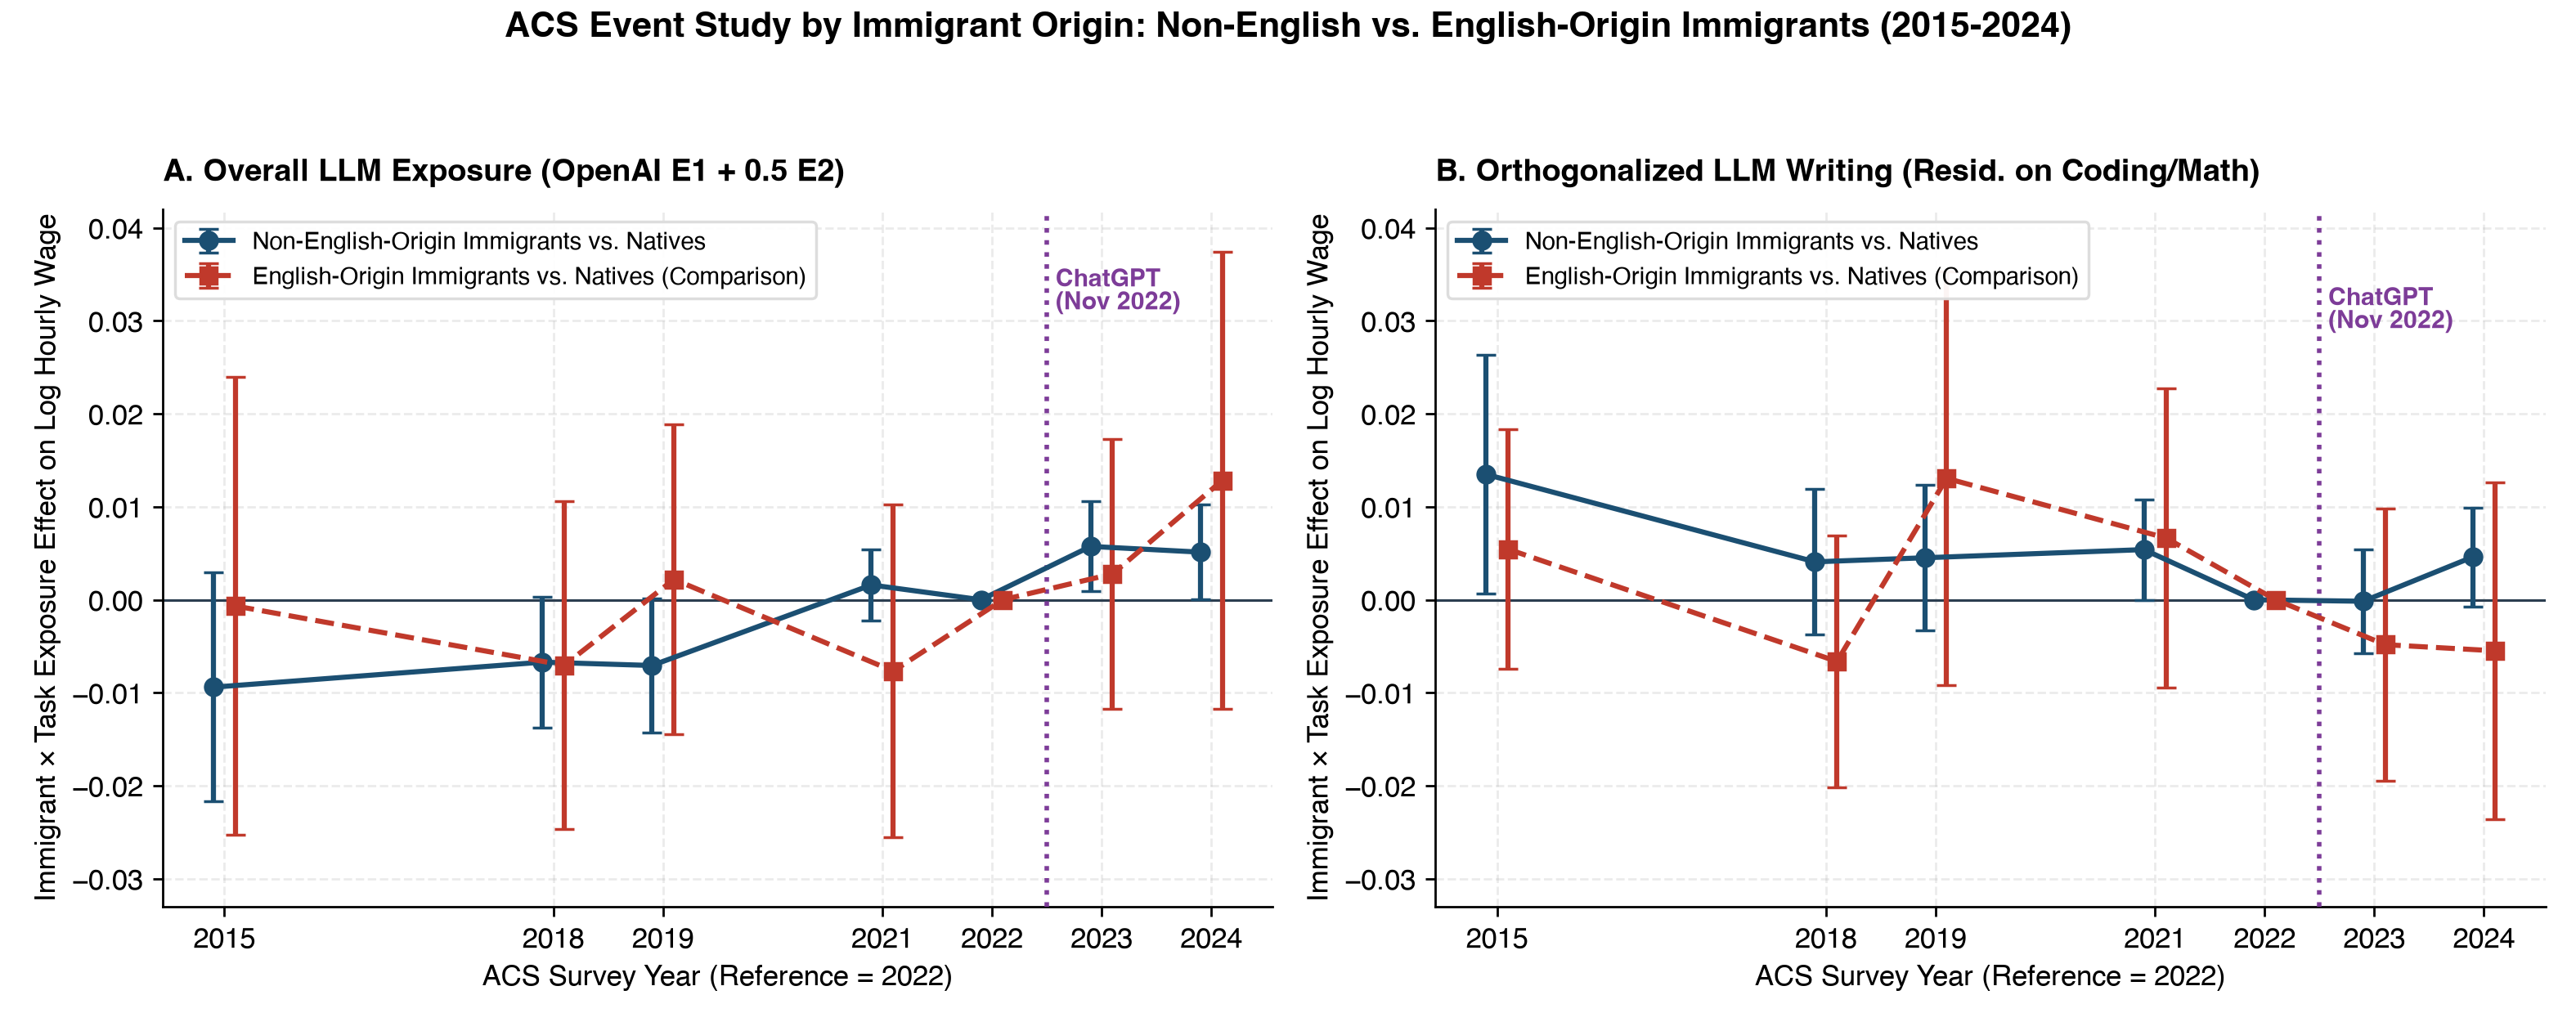
\includegraphics[width=0.86\linewidth,height=0.25\textheight,keepaspectratio]{figures/fig2_acs_eng_vs_noneng_placebo.png}
\caption{ACS Annual Event Study for Capability-Rubric Exposure by Immigrant Origin, 2015--2024. \normalfont Using Eloundou et al.\ (2024) GPT-4 capability scores (reference year $= 2022$), the event study tracks relative log-wage paths for non-English-origin and English-origin immigrants against U.S.-born workers, showing steady pre-2022 upward drift.}
\label{fig:acs_placebo}
\end{figure}

{\renewcommand{\arraystretch}{0.90}\begin{table}[htbp]
\centering
\caption{Simultaneous Task Horse Race: LLM Writing vs.\ LLM Coding/Math vs.\ Face-to-Face Social Skills}
\label{tab:task_horserace}
\footnotesize
\setlength{\tabcolsep}{4pt}
\resizebox{\textwidth}{!}{%
\begin{tabular}{lcccccc}
\toprule
 & \shortstack{(1) Full\\2015--24} & \shortstack{(2) Post-COVID\\2021--24} & \shortstack{(3) OpenAI $\beta$\\2021--24} & \shortstack{(4) OpenAI $E1$\\2021--24} & \shortstack{(5) Felten LM\\2021--24} & \shortstack{(6) Immi-Only\\DDD 2021--24} \\
\midrule
Post $\times$ Treat $\times$ LLM Writing (Orth.) & -0.0006 & 0.0003 & --- & --- & --- & 0.0092 \\
 & (0.0027) & (0.0026) &  &  &  & (0.0064) \\
Post $\times$ Treat $\times$ LLM Coding \& Math & 0.0083*** & 0.0042*** & --- & --- & --- & -0.0110* \\
 & (0.0016) & (0.0015) &  &  &  & (0.0060) \\
Post $\times$ Treat $\times$ OpenAI LLM $\beta$ & --- & --- & 0.0049*** & --- & --- & --- \\
 &  &  & (0.0015) &  &  &  \\
Post $\times$ Treat $\times$ OpenAI LLM $E1$ & --- & --- & --- & 0.0029** & --- & --- \\
 &  &  &  & (0.0014) &  &  \\
Post $\times$ Treat $\times$ Felten LM AIOE & --- & --- & --- & --- & 0.0048** & --- \\
 &  &  &  &  & (0.0021) &  \\
Post $\times$ Treat $\times$ Face-to-Face Social & 0.0005 & -0.0012 & -0.0013 & 0.0007 & -0.0028 & -0.0147*** \\
 & (0.0044) & (0.0044) & (0.0041) & (0.0043) & (0.0043) & (0.0043) \\
\midrule
Workers ($N$) & 6,458,113 & 3,788,812 & 3,788,812 & 3,788,812 & 3,788,812 & 655,697 \\
Cells & 1,705,990 & 1,004,872 & 1,004,872 & 1,004,872 & 1,004,872 & 347,743 \\
$R^2$ & 0.683 & 0.677 & 0.677 & 0.676 & 0.677 & 0.604 \\
SE Clustering & Two-way & Two-way & Two-way & Two-way & Two-way & Two-way \\
Comparison Group & \multicolumn{5}{c}{Non-English-Origin Immigrants vs.\ U.S.\ Natives} & NonEng vs.\ Eng \\
Fixed Effects & \multicolumn{6}{c}{$\text{OCCSOC}\times\text{Year}$, $\text{State}\times\text{Year}$, $\text{Educ4}\times\text{Year}$, $\text{Origin}\times\text{Year}$, $\text{Sex}\times\text{Year}$} \\
\bottomrule
\end{tabular}%
}
\vspace{4pt}
\begin{minipage}{\textwidth}\scriptsize
\textit{Notes:} Each column estimates a single simultaneous regression competing multiple occupation task exposures interacted with $\text{Treat}$ and $\text{Post} = \mathbf{1}[\text{Year}\ge 2023]$. Columns (1)--(5) compare Non-English-origin immigrants to U.S.\ natives; Column (6) restricts the sample to foreign-born immigrants only (Non-English-origin vs.\ English-origin). Because \texttt{LLM Writing (Orth.)} is the OLS residual of \texttt{LLM Writing} on \texttt{LLM Coding \& Math}, it has exact zero correlation with \texttt{LLM Coding \& Math} across occupations. Exact logged SE clustering (\texttt{OCCSOC} + state two-way CRV1, or one-way \texttt{OCCSOC} if a finite-sample two-way diagonal is non-positive) is reported explicitly for each column. $^{***}p<0.01$, $^{**}p<0.05$, $^{*}p<0.10$.
\end{minipage}
\end{table}
}

\begin{figure}[htbp]
\centering
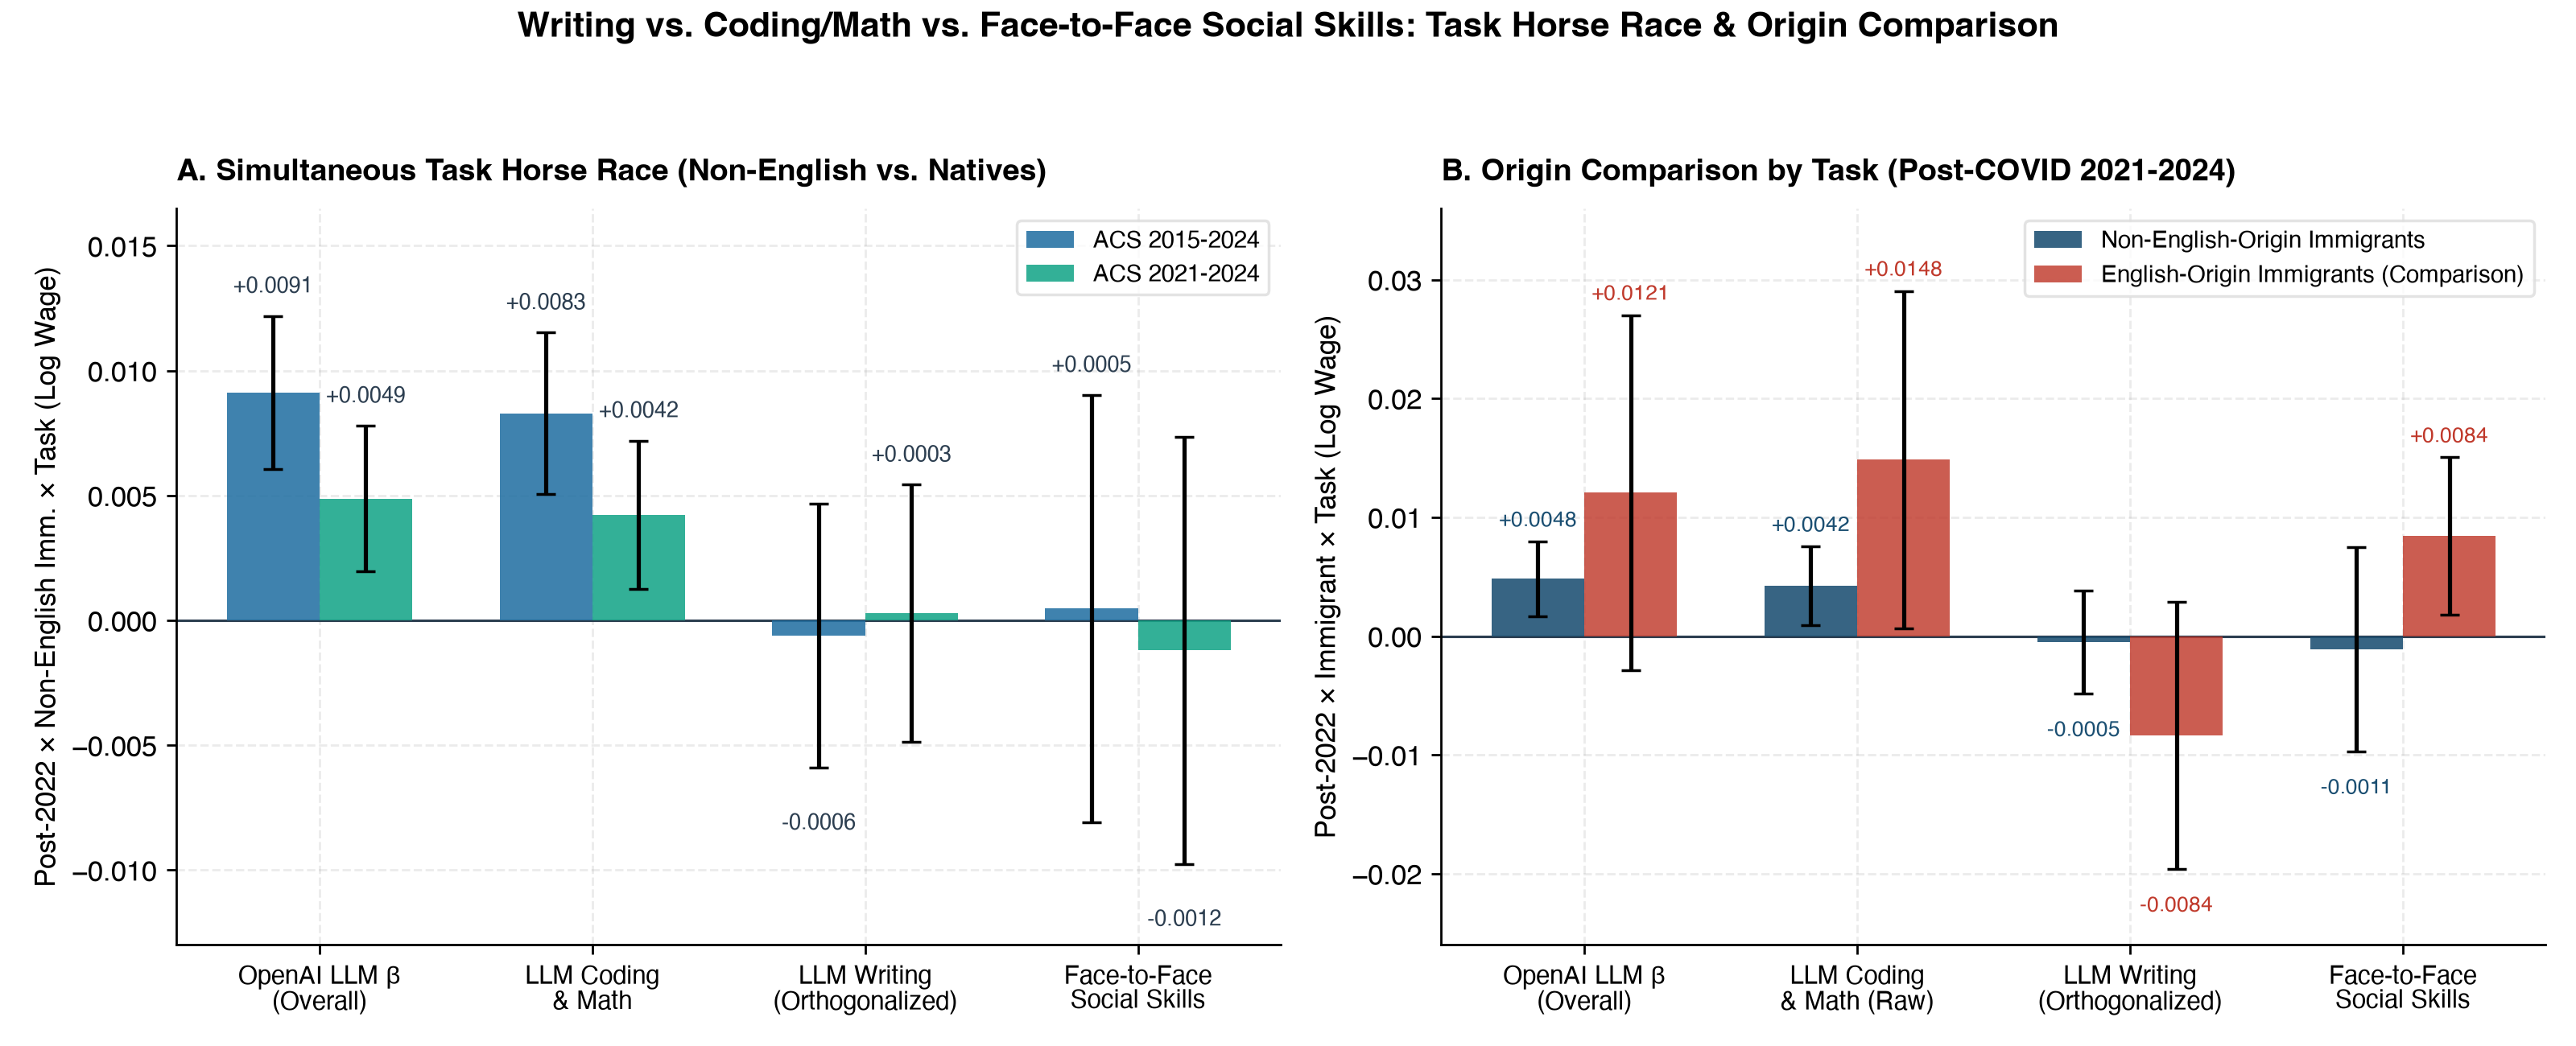
\includegraphics[width=0.86\linewidth,height=0.25\textheight,keepaspectratio]{figures/fig3_writing_vs_coding_vs_social.png}
\caption{Simultaneous Task Horse Race: Written-English, Coding/Math, and Face-to-Face Social Exposure. \normalfont Panel~A competes orthogonalized written-English exposure, coding/math exposure, and face-to-face social skills simultaneously in the ACS; Panel~B compares post-COVID 2021--2024 estimates by immigrant origin.}
\label{fig:horserace}
\end{figure}

A notable contrary result across surveys emerges for face-to-face social skills. In the 2021--2024 individual-worker ACS (Table~\ref{tab:acs_origin_placebo}), non-English-origin immigrants show $-0.0012$ (SE $0.0044$, $p = 0.789$) against $+0.0086^{**}$ (SE $0.0034$) for English-origin immigrants (triple-difference $-0.0097^{**}$, $p = 0.011$). In the CPS (Table~\ref{tab:cps_quarterly_did}), by contrast, non-English-origin immigrants post statistically significant positive wage gains in face-to-face social occupations: $+0.0145^{***}$ (SE $0.0045$, $p = 0.002$) in 2023--2024 and $+0.0115^{**}$ (SE $0.0051$, $p = 0.028$) in 2025--2026. Over the same periods, English-origin immigrants record negative estimates ($-0.0247^{*}$ and $-0.0259$), yielding positive CPS triple-differences of $+0.0393^{***}$ ($p = 0.002$) in 2023--2024 and $+0.0374^{*}$ ($p = 0.058$) in 2025--2026. This cross-survey divergence likely reflects tight post-pandemic service-sector labor markets and compositional differences between CPS weekly earnings and ACS annual FTFY hourly wages, cautioning against attributing ACS social-skill contrasts to a universal native-English communication premium.

{\renewcommand{\arraystretch}{0.90}\begin{table}[htbp]
\centering
\caption{CPS ORG Quarterly Difference-in-Differences, Post-2024 Persistence, and 80\% MDEs (2020 Q1--2026 Q3)}
\label{tab:cps_quarterly_did}
\footnotesize
\setlength{\tabcolsep}{4pt}
\resizebox{\textwidth}{!}{%
\begin{tabular}{lccccccc}
\toprule
 & \multicolumn{2}{c}{Non-English Origin} & 80\% MDE & \multicolumn{2}{c}{English Origin (Comp.)} & \multicolumn{2}{c}{DDD (NonEng $-$ Eng)} \\
\cmidrule(lr){2-3} \cmidrule(lr){5-6} \cmidrule(lr){7-8}
Task / Wage Harmonization & Early & Mature & (Mature & Early & Mature & Early & Mature \\
 & (2023--24) & (2025--26) & Non-Eng) & (2023--24) & (2025--26) & (2023--24) & (2025--26) \\
\midrule
\multicolumn{8}{l}{\textit{Panel A: Task Decomposition (Harmonized Capped Weekly Wage, \$2,884.61 cap)}} \\
\addlinespace[3pt]
O*NET 31.0 Written-English & 0.0080* & 0.0041 & 0.0133 & -0.0138 & -0.0069 & 0.0219 & 0.0111 \\
 & (0.0043) & (0.0048) & & (0.0197) & (0.0209) & (0.0187) & (0.0219) \\
OpenAI LLM Exposure ($E1+0.5\,E2$) & 0.0037 & 0.0059 & 0.0131 & -0.0085 & 0.0312* & 0.0122 & -0.0253 \\
 & (0.0043) & (0.0047) & & (0.0174) & (0.0162) & (0.0183) & (0.0181) \\
LLM Writing (Orthogonalized) & 0.0030 & 0.0041 & 0.0154 & -0.0087 & 0.0151 & 0.0117 & -0.0110 \\
 & (0.0058) & (0.0055) & & (0.0282) & (0.0155) & (0.0283) & (0.0171) \\
LLM Coding \& Math (Raw) & 0.0045 & 0.0050 & 0.0122 & -0.0041 & 0.0190 & 0.0086 & -0.0141 \\
 & (0.0042) & (0.0043) & & (0.0150) & (0.0173) & (0.0162) & (0.0190) \\
Face-to-Face Social Skills & 0.0145*** & 0.0115** & 0.0143 & -0.0247* & -0.0259 & 0.0393*** & 0.0374* \\
 & (0.0045) & (0.0051) & & (0.0133) & (0.0186) & (0.0130) & (0.0197) \\
\midrule
\multicolumn{8}{l}{\textit{Panel B: April 2023 CPS Top-Code Harmonization Robustness (OpenAI LLM $\beta$)}} \\
\addlinespace[3pt]
Log Weekly Wage (Q93 Winsorized) & 0.0046 & 0.0079 & 0.0136 & -0.0061 & 0.0392** & 0.0107 & -0.0313* \\
 & (0.0043) & (0.0049) & & (0.0176) & (0.0161) & (0.0184) & (0.0178) \\
Log Hourly Wage (Harmonized Cap) & 0.0013 & 0.0018 & 0.0124 & -0.0035 & 0.0186 & 0.0049 & -0.0168 \\
 & (0.0039) & (0.0044) & & (0.0163) & (0.0131) & (0.0182) & (0.0142) \\
Log Weekly Wage (Uncapped Raw) & 0.0089* & 0.0116* & 0.0172 & 0.0062 & 0.0683*** & 0.0027 & -0.0567*** \\
 & (0.0052) & (0.0062) & & (0.0184) & (0.0172) & (0.0193) & (0.0182) \\
\midrule
Observations ($N$) & \multicolumn{7}{c}{609,306 FT wage earners (26 quarters, excl.\ transition 2022 Q4); $R^2 = 0.475$} \\
Clusters (OCC2018 / State) & \multicolumn{7}{c}{524 2018 Census occupations / 51 states (two-way CRV1 (OCC2018 + state) in all rows)} \\
Fixed Effects & \multicolumn{7}{c}{$\text{OCC2018}\times\text{YQ}$, $\text{State}\times\text{YQ}$, $\text{Educ4}\times\text{YQ}$, $\text{Origin}\times\text{YQ}$, $\text{Sex}\times\text{YQ}$} \\
\bottomrule
\end{tabular}%
}
\vspace{4pt}
\begin{minipage}{\textwidth}\scriptsize
\textit{Notes:} Sample is full-time wage earners aged 18--64 in 81 Census Basic Monthly CPS ORG files spanning Jan 2020--Oct 2026 (Oct 2025 is missing from Census releases due to the federal shutdown, leaving 2025 Q4 with two months; partial 2026 Q4 and transition quarter 2022 Q4 are excluded), weighted by \texttt{EARNWT}. Pre-period is 2020 Q1--2022 Q3; Early GenAI is 2023 Q1--2024 Q4; Mature GenAI is 2025 Q1--2026 Q3. Column ``80\% MDE'' reports $2.8016 \times \text{SE}$ for Mature Non-English-origin estimates. Note the positive CPS Face-to-Face Social estimates for Non-English-origin immigrants ($+0.0145^{***}$ in 2023--24, $+0.0115^{**}$ in 2025--26, DDD $+0.0393^{***}$), discussed in Section 5. Standard errors in parentheses. $^{***}p<0.01$, $^{**}p<0.05$, $^{*}p<0.10$.
\end{minipage}
\end{table}
}

\begin{figure}[htbp]
\centering
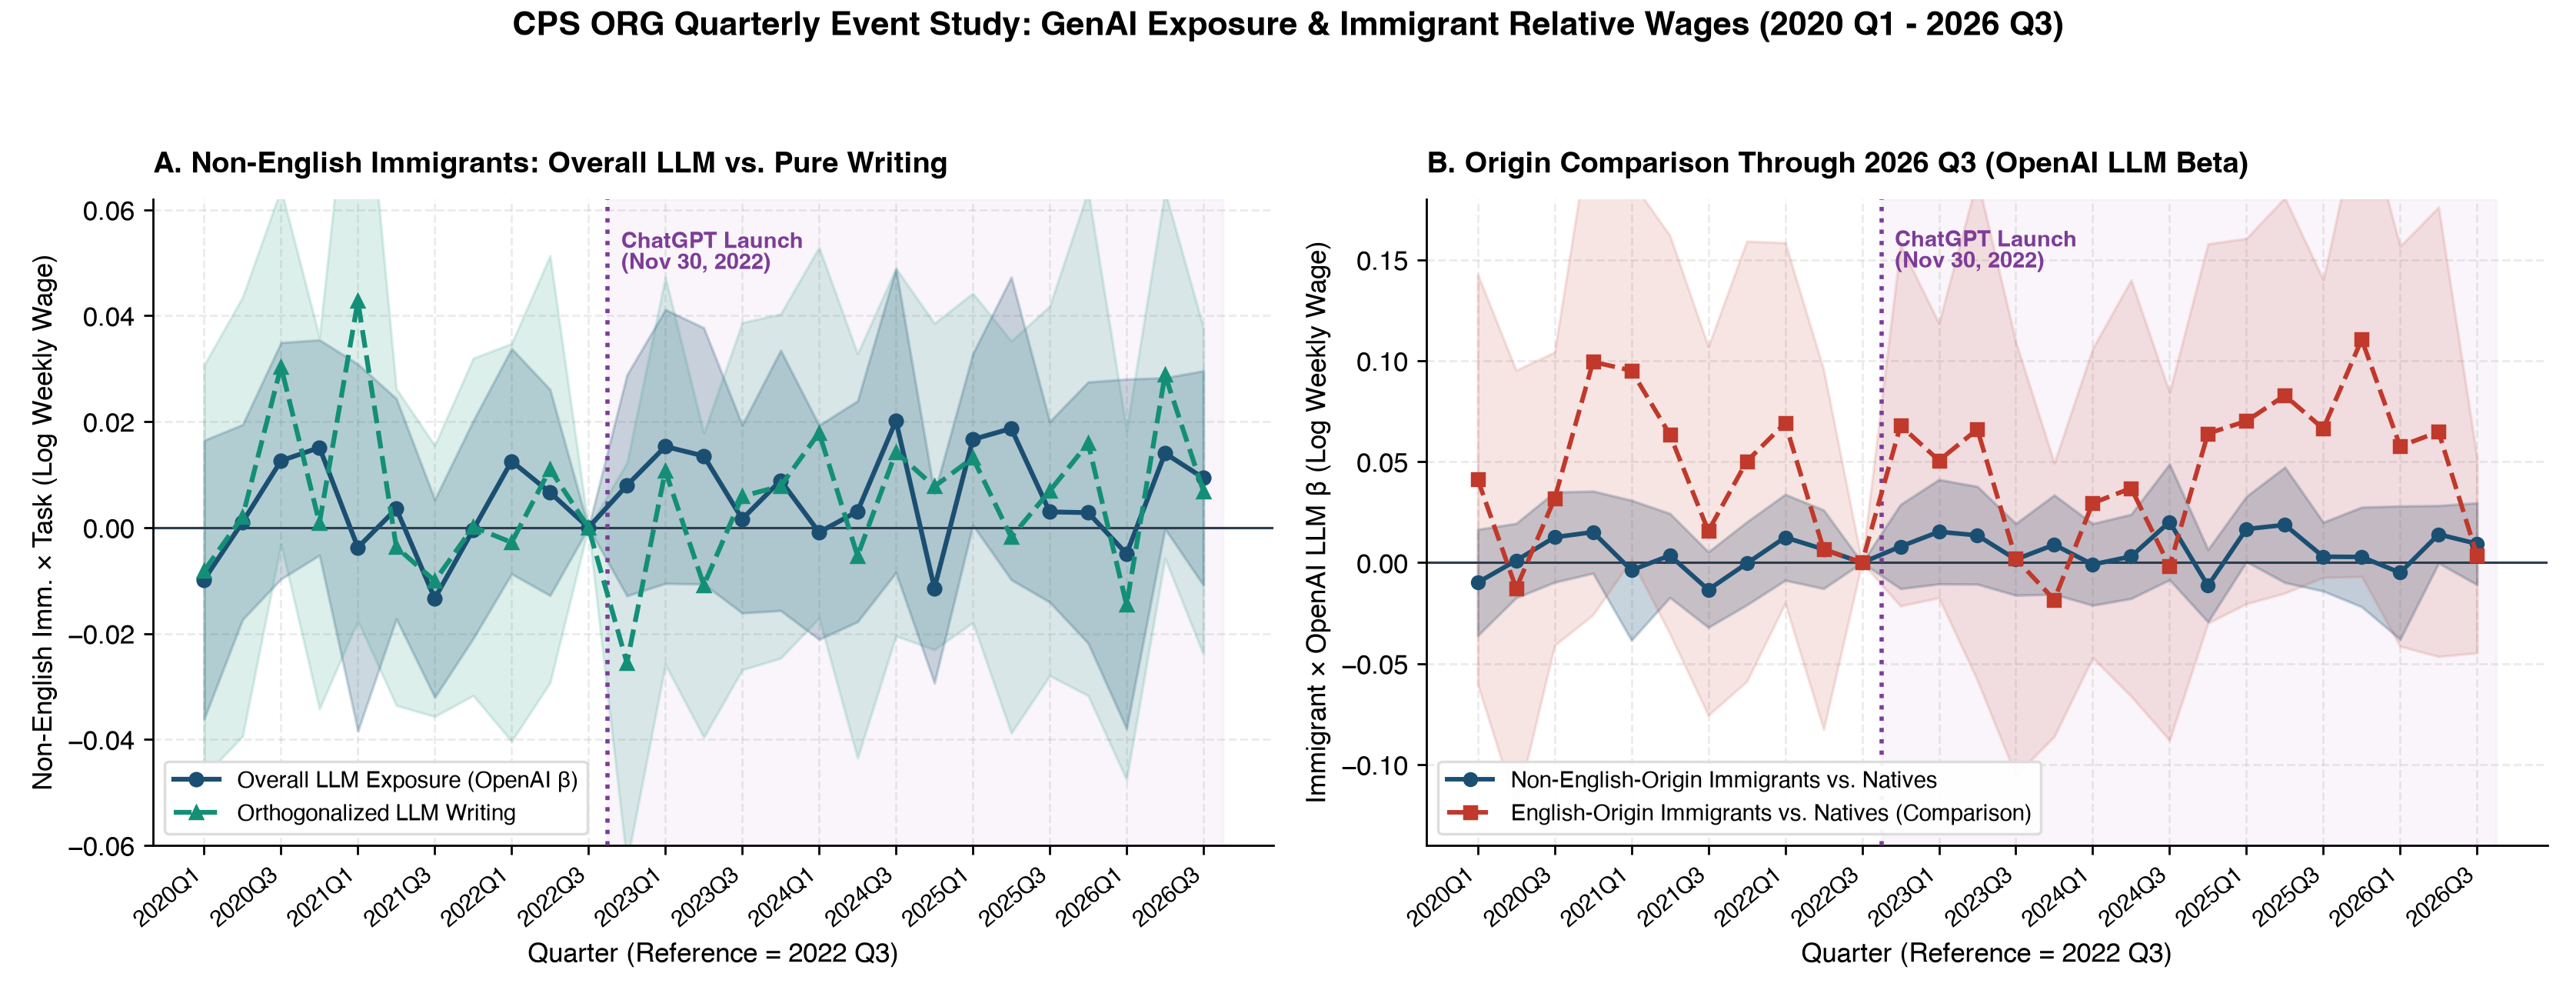
\includegraphics[width=0.88\linewidth,height=0.25\textheight,keepaspectratio]{figures/fig1_cps_quarterly_event_study.png}
\caption{Harmonized Quarterly CPS Earnings Event Study by Immigrant Origin, 2020 Q1--2026 Q3. \normalfont Tracks quarterly relative weekly earnings under the uniform \$2,884.61 cap using Eloundou et al.\ (2024) exposure (reference quarter $= 2022$ Q3), showing flat non-English-origin trajectories alongside a 2025--2026 surge among English-origin immigrants.}
\label{fig:cps_es}
\end{figure}

Table~\ref{tab:cps_quarterly_did} Panel~B and Figure~\ref{fig:cps_es} also document the April 2023 \citet{CensusBLS2023} top-code distortion and quarterly earnings trajectories. On uniformly capped CPS weekly earnings ($\$2{,}884.61$), OpenAI $\beta$ yields insignificant estimates ($+0.0037$, SE $0.0043$ in 2023--2024; $+0.0059$, SE $0.0047$ in 2025--2026, 80 percent MDE $0.0131$), with O*NET 31.0 written-English intensity showing $+0.0080^{*}$ ($p = 0.067$) in 2023--2024 and $+0.0041$ ($p = 0.388$) in 2025--2026. Running the same regression on raw uncapped weekly earnings mechanically doubles the non-English estimate to $+0.0089^{*}$ (2023--2024) and $+0.0116^{*}$ (2025--2026) and inflates the English-origin estimate to $+0.0683^{***}$.

{\renewcommand{\arraystretch}{0.90}\begin{table}[htbp]
\centering
\caption{Exploratory Plug-In LP Pre-Trend Bounds and ACS Heterogeneity (2021--2024)}
\label{tab:robustness_honestdid}
\footnotesize
\setlength{\tabcolsep}{4pt}
\resizebox{\textwidth}{!}{%
\begin{tabular}{lcccc}
\toprule
\multicolumn{5}{l}{\textit{Panel A: Exploratory Plug-In LP Pre-Trend Bounds (Time-Scaled 95\% FLCIs, Non-English Immigrants vs.\ Natives)}} \\
\addlinespace[3pt]
Pre-Trend Bound ($\bar{M}$) & ACS OpenAI LLM $\beta$ & ACS LLM Writing (Orth.) & CPS OpenAI $\beta$ (2023--24) & CPS OpenAI $\beta$ (2023--26) \\
\midrule
Point Est.\ $\hat{\theta}$ (SE) & 0.0054 (0.0023) & 0.0022 (0.0019) & 0.0063 (0.0087) & 0.0073 (0.0081) \\
\addlinespace[2pt]
$\bar{M} = 0.0$ & [+0.0010,\; +0.0099] & [-0.0015,\; +0.0059] & [-0.0108,\; +0.0234] & [-0.0086,\; +0.0233] \\
$\bar{M} = 0.5$ & [-0.0015,\; +0.0124] & [-0.0049,\; +0.0094] & [-0.0547,\; +0.0672] & [-0.0823,\; +0.0969] \\
$\bar{M} = 1.0$ & [-0.0048,\; +0.0156] & [-0.0090,\; +0.0134] & [-0.1012,\; +0.1138] & [-0.1585,\; +0.1731] \\
$\bar{M} = 1.5$ & [-0.0080,\; +0.0189] & [-0.0130,\; +0.0175] & [-0.1478,\; +0.1604] & [-0.2347,\; +0.2494] \\
$\bar{M} = 2.0$ & [-0.0113,\; +0.0221] & [-0.0171,\; +0.0215] & [-0.1944,\; +0.2070] & [-0.3109,\; +0.3256] \\
\midrule
\multicolumn{5}{l}{\textit{Panel B: ACS 2021--2024 Heterogeneity (Non-English-Origin Immigrants vs.\ U.S.\ Natives)}} \\
\addlinespace[3pt]
Subgroup & \multicolumn{2}{c}{OpenAI LLM $\beta$ (SE)} & \multicolumn{2}{c}{LLM Writing Orth.\ (SE) / $N$ Workers} \\
\midrule
Fluent English (SPEAKENG 3-4) & 0.0055*** & (0.0020) & -0.0016 (0.0021) & 3,553,671 \\
Non-Fluent English (SPEAKENG 1,5,6) & -0.0008 & (0.0042) & 0.0002 (0.0050) & 3,419,487 \\
College STEM (DEGFIELD STEM) & 0.0054 & (0.0065) & -0.0002 (0.0057) & 416,175 \\
College Non-STEM & 0.0093* & (0.0048) & -0.0037 (0.0040) & 1,278,607 \\
Non-College ($<$ BA) & 0.0029 & (0.0032) & 0.0046 (0.0046) & 2,094,030 \\
Men & 0.0049* & (0.0025) & 0.0019 (0.0042) & 2,106,999 \\
Women & 0.0048* & (0.0027) & -0.0025 (0.0028) & 1,681,813 \\
Young (18-34) & 0.0062*** & (0.0020) & -0.0077 (0.0065) & 1,078,168 \\
Prime-Age (35-49) & 0.0055* & (0.0030) & 0.0005 (0.0034) & 1,377,941 \\
Senior (50-64) & 0.0009 & (0.0024) & 0.0017 (0.0058) & 1,332,703 \\
Recent Arrivals ($<$10 yrs) & 0.0070 & (0.0043) & 0.0023 (0.0065) & 3,307,059 \\
Established ($\ge$10 yrs) & 0.0028 & (0.0018) & -0.0015 (0.0030) & 3,666,099 \\
\bottomrule
\end{tabular}%
}
\vspace{4pt}
\begin{minipage}{\textwidth}\scriptsize
\textit{Notes:} Panel A reports exploratory plug-in pre-trend sensitivity bounds computed via a Python linear program (\texttt{scipy.optimize.linprog}, HiGHS) inspired by \citet{RambachanRoth2023} relative-magnitude restrictions ($\Delta^{\text{RM}}(\bar{M})$), using bias-aware folded-normal critical values $\text{cv}_{0.05}(b_{\max}/\hat{\sigma})$ and explicit per-period time-step scaling for uneven ACS calendar years and quarterly CPS steps (accounting for the omitted 2022 Q4 transition quarter). Because solving the LP at the plug-in maximum pre-trend slope does not account for sampling uncertainty in the estimated pre-trend, these intervals should be read as exploratory sensitivity diagnostics awaiting benchmarking against the official R \texttt{HonestDiD} package. $\bar{M}=0$ imposes exact parallel trends; $\bar{M}=1$ allows post-treatment per-period trend slopes as large as the maximum plug-in pre-treatment per-period slope. Panel B estimates the baseline ACS 2021--2024 specification separately by subgroup with two-way clustered SEs (\texttt{OCCSOC} + state). $^{***}p<0.01$, $^{**}p<0.05$, $^{*}p<0.10$.
\end{minipage}
\end{table}
}

Finally, Table~\ref{tab:robustness_honestdid} and Figure~\ref{fig:honestdid} present our exploratory plug-in LP pre-trend bounds and ACS subgroup splits. The ACS event-study post-period average relative to 2022 alone is $\frac{1}{2}(\hat{\beta}_{2023} + \hat{\beta}_{2024}) = +0.0054$ (SE $0.0023$) for OpenAI $\beta$, a distinct estimand from the pooled 2021--2024 difference-in-differences estimate of $+0.0048$ (which averages 2021 and 2022 in the pre-period). Under our exploratory plug-in LP bounds with actual calendar-year intervals ($[3, 1, 2, 1]$ pre-2022 and $[1, 1]$ post-2022), the 95 percent FLCI for OpenAI $\beta$ excludes zero only under exact parallel trends ($\bar{M} = 0$: $[+0.0010, +0.0099]$) and crosses zero at $\bar{M} = 0.5$ ($[-0.0015, +0.0124]$). For AEI 2026 Observed (event-study average $+0.0006$, SE $0.0013$), the 95 percent FLCI includes zero even at $\bar{M} = 0$ ($[-0.0020, +0.0032]$; $[-0.0042, +0.0055]$ at $\bar{M} = 0.5$). Subgroup splits (Table~\ref{tab:robustness_honestdid}, Panel~B) show that the modest OpenAI $\beta$ gain concentrates among fluent English speakers ($+0.0055^{***}$), non-STEM college graduates ($+0.0093^{*}$, versus an insignificant $+0.0054$ for STEM college graduates), and workers aged 18--34 ($+0.0062^{***}$), rather than non-fluent workers ($-0.0008$, $p = 0.844$). CPS occupational entry through 2026 Q3 likewise shows no post-2022 surge of non-English-origin immigrants into top-quartile AI occupations ($-1.22$ pp$^{***}$ in 2023--2024; $-0.09$ pp, $p = 0.723$ in 2025--2026).

\begin{figure}[htbp]
\centering
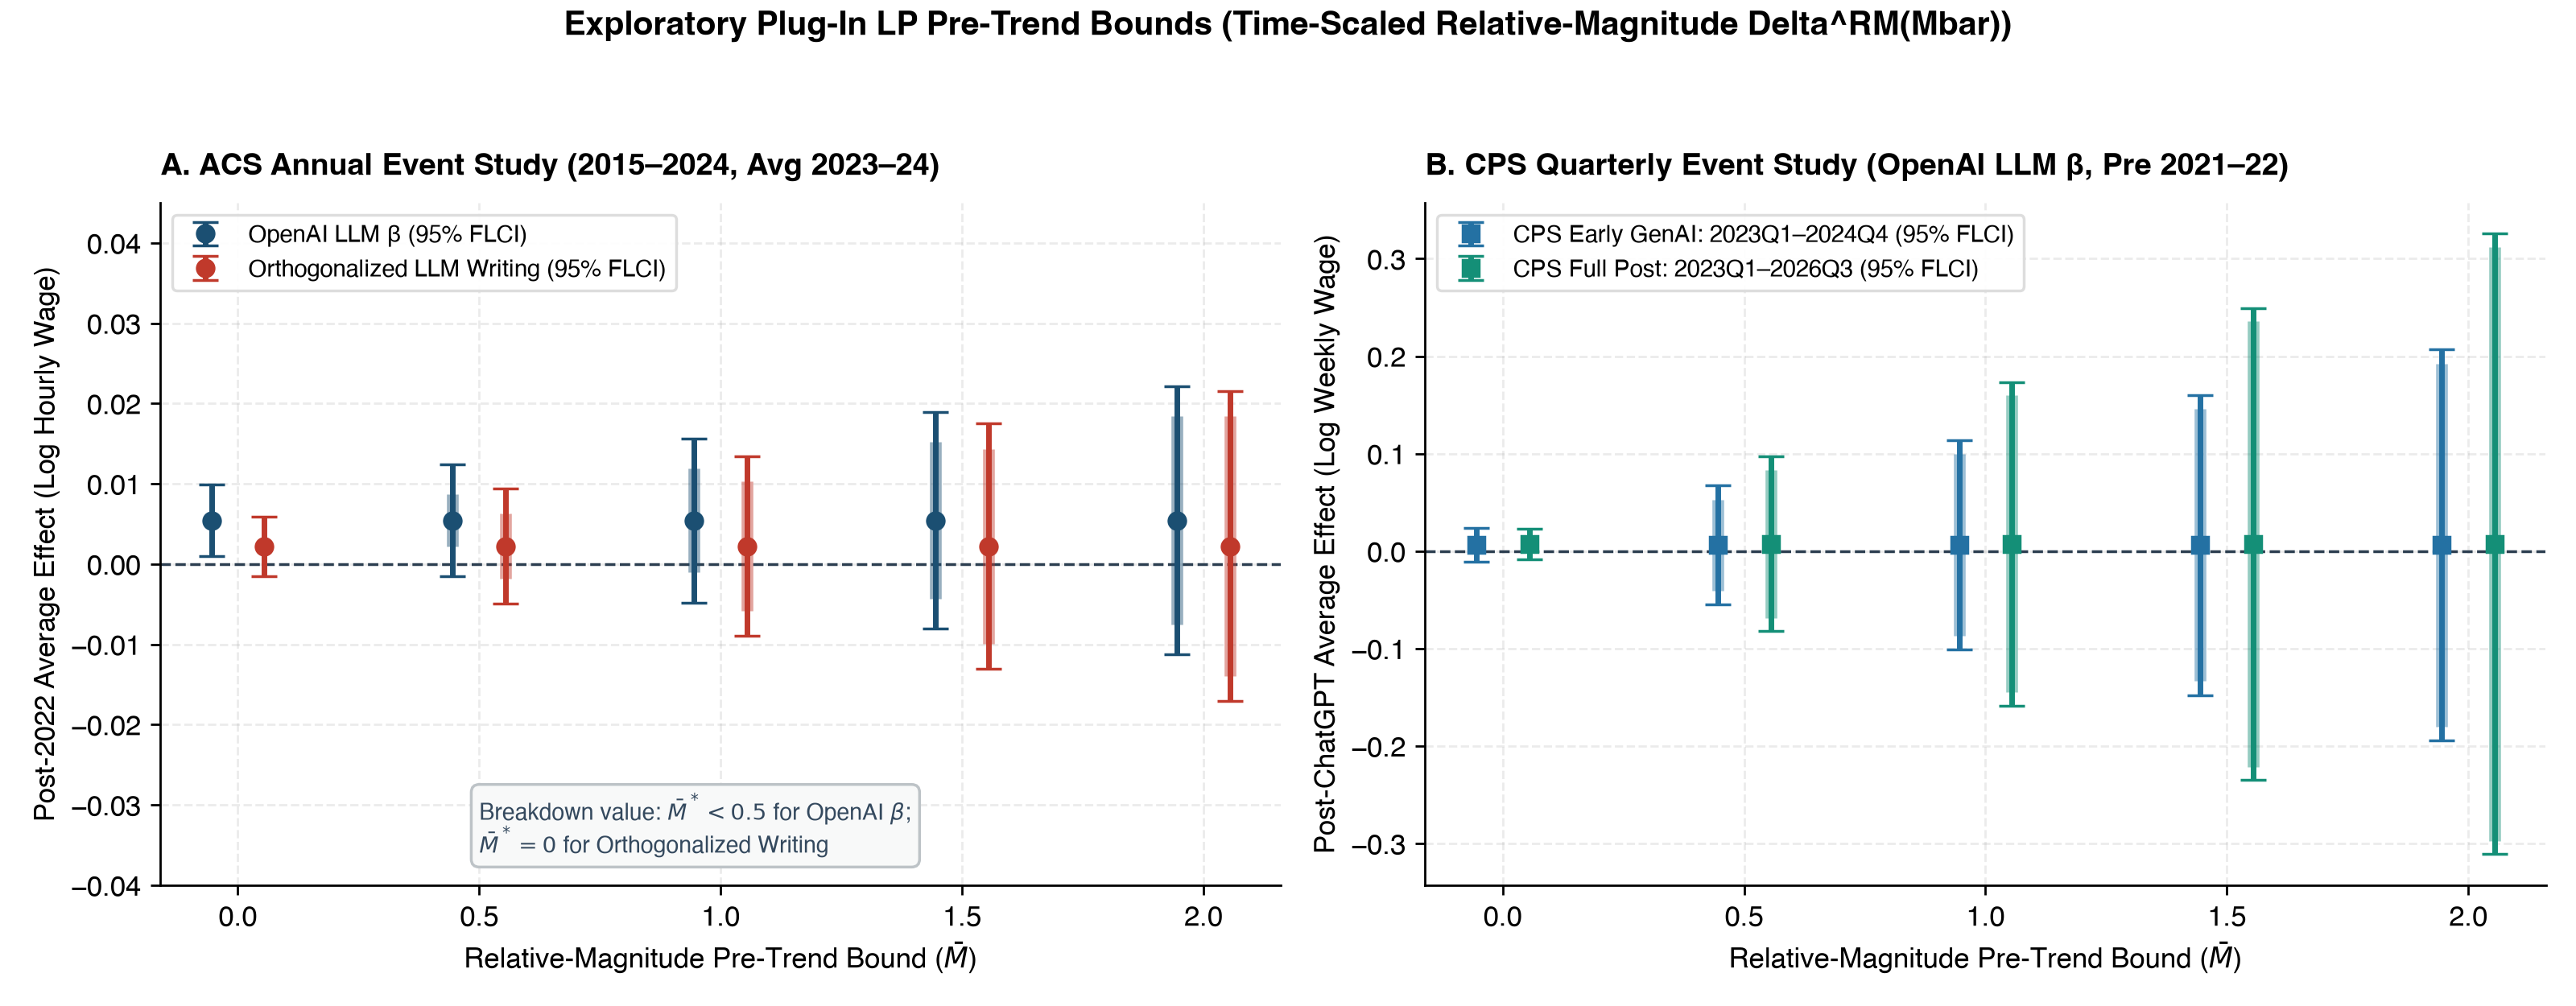
\includegraphics[width=0.88\linewidth,height=0.25\textheight,keepaspectratio]{figures/fig4_honestdid_sensitivity.png}
\caption{Exploratory Plug-In Linear-Programming Pre-Trend Sensitivity Bounds Across $\bar{M} \in [0, 2]$. \normalfont Plots 95 percent bias-aware FLCIs and plug-in LP identified sets under relative-magnitude restrictions ($\Delta^{\text{RM}}(\bar{M})$) with explicit calendar-time step scaling for uneven ACS years and quarterly CPS intervals.}
\label{fig:honestdid}
\end{figure}

\section{Limitations and Scope}\label{sec:limitations}

Several methodological boundaries govern interpretation of these findings. First, because origin-by-time and occupation-by-time fixed effects absorb economy-wide immigrant-level wage shifts and occupation-level shocks, our estimates and MDEs apply strictly to differential wage changes \emph{across occupations by measured exposure}; they do not bound uniform economy-wide gains across all jobs or gains realized through occupational mobility.

Second, every available exposure measure carries timing and measurement limitations. O*NET 31.0 (2026 release) task ratings are refreshed on rolling cycles and cannot be treated as strictly pre-launch predetermined without an archived pre-2022 vintage; \citet{Eloundou2024} was constructed in early 2023 from GPT-4 capabilities; and March 2026 AEI observed exposure \citep{MassenkoffMcCrory2026} is measured post-treatment from single-provider Claude telemetry ($54.3$ percent zeros), creating attenuation toward zero. In addition, 2023 ACS annual wage income covers the preceding 12 months, so part of 2023 ACS earnings precedes ChatGPT's November 2022 launch.

Third, statistical power differs sharply across surveys. While the 2021--2024 ACS rules out occupational-exposure gradients larger than $0.0027\text{--}0.0047$ log points per SD under AEI 2026 exposure ($0.0045\text{--}0.0084$ log points under capability rubrics and O*NET 31.0), the 2025--2026 CPS has 80 percent MDEs of $0.0114\text{--}0.0171$ log points per SD and therefore cannot rule out modest post-2024 gradients. Furthermore, solving our time-scaled plug-in LP at the maximum pre-trend slope does not incorporate sampling uncertainty in the estimated pre-trend; those bounds remain exploratory diagnostics awaiting benchmarking against official \texttt{HonestDiD} inference.

Finally, two empirical caveats caution against over-interpreting subgroup contrasts. Because English-speaking-origin immigrants are differentially selected into finance and technology (loading onto coding in the ACS and flipping from $-0.0062$ in 2023--2024 to $+0.0286^{***}$ in 2025--2026 across roughly $1{,}565$ CPS earners), triple-difference contrasts against this group should be read as selection diagnostics rather than causal placebo tests. Likewise, the positive CPS estimates for face-to-face social skills ($+0.0145^{***}$ and $+0.0115^{**}$) diverge from the flat ACS estimate ($-0.0012$), underscoring sensitivity to earnings definitions and sample composition, while March 2025 automation and augmentation shares \citep{Handa2025} represent interim snapshots predating 2026 agentic shifts \citep{Appel2026, Massenkoff2026a, Massenkoff2026b}.

\FloatBarrier
\section{Conclusion}

Across $6.55$ million individual full-time workers in the 2015--2024 ACS and $634{,}326$ full-time earners tracked quarterly through 2026 Q3 in the CPS ORG, we find no detectable differential wage equalization along measured occupational AI exposure for non-English-origin immigrants so far. In authoritative individual-worker 2021--2024 ACS regressions, relative wage gradients are small and statistically indistinguishable from zero across O*NET 31.0 written-English intensity, orthogonalized written-English AI exposure, and observed March 2026 Claude usage. Modest positive estimates on early-2023 OpenAI capability scores load onto coding and quantitative work rather than writing and lose statistical significance once modest pre-trend continuation is permitted under exploratory plug-in LP bounds. In the harmonized CPS through late 2026, estimates remain statistically insignificant, ruling out large occupational-gradient equalization ($>1.5\text{--}2$ percent per SD) while leaving smaller effects unresolved.

These findings align with emerging administrative evidence from Denmark and Finland documenting rapid workplace AI adoption alongside small or null early aggregate wage responses \citep{HumlumVestergaard2025, KauhanenRouvinen2025}, and indicate that experimental and online-freelancing writing gains \citep{NoyZhang2023, Dalaman2025, CaoLi2025SSRN} have not yet materialized as broad cross-occupation wage compression in U.S.\ wage surveys. Whether multi-provider adoption data, archived pre-2022 O*NET vintages, longer adjustment horizons, or real-time voice-translation tools alter this pattern remains an important question for future research.

\section*{Acknowledgments}
This research was directed by Daksh Tyagi and carried out by a swarm of Gemini 4 Neon agents. All empirical specifications, individual-worker replications, end-to-end crosswalk builds, and manuscript revisions were audited against the underlying Census CPS, IPUMS ACS, O*NET 31.0, and Anthropic Economic Index public-use data files.

\FloatBarrier
\begin{thebibliography}{99}

\bibitem[Appel et al.(2026)]{Appel2026}
Appel, R., Massenkoff, M., McCrory, P., McCain, M., Heller, R., Neylon, T., and Tamkin, A. (2026). \emph{Anthropic Economic Index report: Economic primitives}. Anthropic Research, January 15, 2026.

\bibitem[Autor and Dorn(2013)]{AutorDorn2013}
Autor, D. H., and Dorn, D. (2013). The growth of low-skill service jobs and the polarization of the US labor market. \emph{American Economic Review}, 103(5), 1553--1597.

\bibitem[Autor, Levy and Murnane(2003)]{AutorLevyMurnane2003}
Autor, D. H., Levy, F., and Murnane, R. J. (2003). The skill content of recent technological change: An empirical exploration. \emph{Quarterly Journal of Economics}, 118(4), 1279--1333.

\bibitem[Brynjolfsson, Li and Raymond(2025)]{Brynjolfsson2025}
Brynjolfsson, E., Li, D., and Raymond, L. (2025). Generative AI at work. \emph{Quarterly Journal of Economics}, 140(2), 889--942.

\bibitem[Cameron, Gelbach and Miller(2011)]{CameronGelbachMiller2011}
Cameron, A. C., Gelbach, J. B., and Miller, D. L. (2011). Robust inference with multiway clustering. \emph{Journal of Business \& Economic Statistics}, 29(2), 238--249.

\bibitem[Cao and Li(2025)]{CaoLi2025SSRN}
Cao, J., and Li, Z. (2025). \emph{AI for fairness? The role of generative tools in shaping freelancer success}. SSRN Working Paper No. 5346514.

\bibitem[Dalaman, Kalay and Kettlewell(2025)]{Dalaman2025}
Dalaman, B., Kalay, A. F., and Kettlewell, N. (2025). \emph{Bridging language barriers: The impact of large language models on academic writing}. IZA Discussion Paper No. 18215, October 2025.

\bibitem[Deming(2017)]{Deming2017}
Deming, D. J. (2017). The growing importance of social skills in the labor market. \emph{Quarterly Journal of Economics}, 132(4), 1593--1640.

\bibitem[Eloundou et al.(2024)]{Eloundou2024}
Eloundou, T., Manning, S., Mishkin, P., and Rock, D. (2024). GPTs are GPTs: Labor market impact potential of LLMs. \emph{Science}, 384(6702), 1306--1308.

\bibitem[Felten, Raj and Seamans(2021)]{Felten2021}
Felten, E., Raj, M., and Seamans, R. (2021). Occupational, industry, and geographic exposure to artificial intelligence: A novel dataset and its potential uses. \emph{Strategic Management Journal}, 42(12), 2195--2217.

\bibitem[Felten, Raj and Seamans(2023)]{Felten2023}
Felten, E., Raj, M., and Seamans, R. (2023). \emph{Occupational heterogeneity in exposure to generative AI}. Working Paper / SSRN 4414065, April 2023.

\bibitem[Handa et al.(2025)]{Handa2025}
Handa, K., Tamkin, A., McCain, M., Huang, S., Durmus, E., Heck, S., Mueller, J., Hong, J., Ritchie, S., Belonax, T., Troy, K. K., Amodei, D., Kaplan, J., Clark, J., and Ganguli, D. (2025). \emph{Which economic tasks are performed with AI? Evidence from millions of Claude conversations}. arXiv:2503.04761.

\bibitem[Humlum and Vestergaard(2025)]{HumlumVestergaard2025}
Humlum, A., and Vestergaard, E. (2025). \emph{Still waters, rapid currents: Early labor market transformation under generative AI} (originally circulated as \emph{Large language models, small labor market effects}). NBER Working Paper No. 33777, May 2025 (revised March 2026).

\bibitem[Kauhanen and Rouvinen(2025)]{KauhanenRouvinen2025}
Kauhanen, A., and Rouvinen, P. (2025). Assessing early labour market effects of generative AI: Evidence from population data. \emph{Applied Economics Letters}, 33(18), 3471--3474.

\bibitem[Koo(2025)]{Koo2025}
Koo, W. W. (2025). Cross-lingual effects of AI-generated content on human work. \emph{Scientific Reports}, 15, doi:10.1038/s41598-025-16650-w.

\bibitem[Lee(2026)]{Lee2026}
Lee, S. (2026). Occupational exposure to generative AI and worker wages in Korea. \emph{Applied Economics Letters}, published online October 2026.

\bibitem[Massenkoff et al.(2026a)]{Massenkoff2026a}
Massenkoff, M., Lyubich, E., McCrory, P., Appel, R., and Heller, R. (2026a). \emph{Anthropic Economic Index report: Learning curves}. Anthropic Research, March 24, 2026.

\bibitem[Massenkoff et al.(2026b)]{Massenkoff2026b}
Massenkoff, M., Lyubich, E., Sacher, S., Hitzig, Z., Zhang, S., Heller, R., and McCrory, P. (2026b). \emph{Anthropic Economic Index report: Cadences}. Anthropic Research, June 26, 2026.

\bibitem[Massenkoff and McCrory(2026)]{MassenkoffMcCrory2026}
Massenkoff, M., and McCrory, P. (2026). \emph{Labor market impacts of AI: A new measure and early evidence}. Anthropic Research, March 2026.

\bibitem[National Center for O*NET Development(2026)]{ONET2026}
National Center for O*NET Development (2026). \emph{O*NET 31.0 Database}. U.S.\ Department of Labor, Employment and Training Administration.

\bibitem[Noy and Zhang(2023)]{NoyZhang2023}
Noy, S., and Zhang, W. (2023). Experimental evidence on the productivity effects of generative artificial intelligence. \emph{Science}, 381(6654), 187--192.

\bibitem[Peri and Sparber(2009)]{PeriSparber2009}
Peri, G., and Sparber, C. (2009). Task specialization, immigration, and wages. \emph{American Economic Journal: Applied Economics}, 1(3), 135--169.

\bibitem[Rambachan and Roth(2023)]{RambachanRoth2023}
Rambachan, A., and Roth, J. (2023). A more credible approach to parallel trends. \emph{Review of Economic Studies}, 90(5), 2555--2591.

\bibitem[Ruggles et al.(2026)]{Ruggles2026}
Ruggles, S., Flood, S., Sobek, M., Backman, D., Chen, A., Cooper, G., Richards, S., Rodgers, R., and Schouweiler, M. (2026). \emph{IPUMS USA: Version 16.0 [dataset]}. Minneapolis, MN: IPUMS. https://doi.org/10.18128/D010.V16.0

\bibitem[Song(2017)]{Song2017}
Song, T. (2017). \emph{Three Essays on Immigrants' Socio-Economic Integration in the United States}. Ph.D.\ Dissertation, Department of Economics, University of Connecticut.

\bibitem[Song(2026)]{Song2026JHC}
Song, T. (2026). Native--immigrant wage gaps and the growing importance of social skills. \emph{Journal of Human Capital}, published online ahead of print, September 2026, doi:10.1086/742703.

\bibitem[U.S.\ Census Bureau / BLS(2023)]{CensusBLS2023}
U.S.\ Census Bureau and Bureau of Labor Statistics (2023). \emph{CPS Earnings Topcoding Methodology Change (April 2023 Dynamic Topcoding)}. U.S.\ Census Bureau and Bureau of Labor Statistics.

\end{thebibliography}

\end{document}
